%%%%%%%%%%%%%%%%%%%%%%%%%%%%% Thesis.tex %%%%%%%%%%%%%%%%%%%%%%%%%%%%%%%
%                                                                      %
%  ---------- Master of Science Dissertation template ----------       %
%                                                                      %
%  Template for the Master Thesis according to the regulations         %
%  published by the Academic Board (Direcção Académica) at IST.        %
%                                                                      %
%  For up-to-date guide, please refer to the offical website           %
%  http://da.tecnico.ulisboa.pt/dissertacao-de-mestrado/               %
%                                                                      %
%       Andre C. Marta                                                 %
%       Area Cientifica de Mecanica Aplicada e Aeroespacial            %
%       Departamento de Engenharia Mecanica                            %
%       Instituto Superior Tecnico                                     %
%       Av. Rovisco Pais                                               %
%       1049-001 Lisboa                                                %
%       Portugal                                                       %
%       Tel: +351 21 841 9469                                          %
%                        3469 (extension)                              %
%       Email: andre.marta@tecnico.ulisboa.pt                          %
%                                                                      %
%  Created:       Jan 20, 2011                                         %
%  Last Modified: Jul  2, 2015                                         %
%                                                                      %
%%%%%%%%%%%%%%%%%%%%%%%%%%%%%%%%%%%%%%%%%%%%%%%%%%%%%%%%%%%%%%%%%%%%%%%%
%  Revision history                                                    %
%  v1 - 2011/01/24 - original template                                 %
%  v2 - 2012/10/30 - new IST image and glossary support                %
%  v3 - 2013/12/10 - update according to 2012/13 official guide        %
%  v4 - 2014/02/28 - new default for bibliography style                %
%  v5 - 2014/05/07 - update according to 2013/14 official guide        %
%  v6 - 2015/07/02 - cover page format fixed,                          %
%                    contents page numbering fixed,                    %
%                    better language support,                          %
%                    enhanced examples of tables,                      %
%                    new option for appendix page numbering format,    %
%                    custom bibliography style                         %
%%%%%%%%%%%%%%%%%%%%%%%%%%%%%%%%%%%%%%%%%%%%%%%%%%%%%%%%%%%%%%%%%%%%%%%%
%                                                                      %
% To generate the PDF file, type "make" at the terminal prompt.        %
%                                                                      %
% The IST template LaTeX package was created by the author             %
% and it can be downloaded from:                                       %
% https://fenix.ist.utl.pt/homepage/ist31052/                          %
%                                                                      %
% The external packages can be downloaded from                         %
% the Comprehensive TeX Archive Network at http://www.ctan.org/        %
%                                                                      %
% List of LaTex symbols:                                               %
% http://www.ctan.org/tex-archive/info/symbols/comprehensive/          %
%                                                                      %
% Help with LaTex can be found at                                      %
% http://www.giss.nasa.gov/tools/latex/ltx-2.html                      %
% http://en.wikibooks.org/wiki/LaTeX                                   %
%%%%%%%%%%%%%%%%%%%%%%%%%%%%%%%%%%%%%%%%%%%%%%%%%%%%%%%%%%%%%%%%%%%%%%%%

%%%%%%%%%%%%%%%%%%%%%%%%%%%%%%%%%%%%%%%%%%%%%%%%%%%%%%%%%%%%%%%%%%%%%%%%
%     Preamble                                                         %
%%%%%%%%%%%%%%%%%%%%%%%%%%%%%%%%%%%%%%%%%%%%%%%%%%%%%%%%%%%%%%%%%%%%%%%%

% ----------------------------------------------------------------------
%  Set the document class
% ----------------------------------------------------------------------
\documentclass[10pt,a4paper,twoside]{report}

% ----------------------------------------------------------------------
% Define external packages, language, margins, fonts and new commands
% ----------------------------------------------------------------------
%%%%%%%%%%%%%%%%%%%%%%%%%%%%%%%%%%%%%%%%%%%%%%%%%%%%%%%%%%%%%%%%%%%%%%%%
%                                                                      %
%     File: Thesis_Preamble.tex                                        %
%     Tex Master: Thesis.tex                                           %
%                                                                      %
%     Author: Andre C. Marta                                           %
%     Last modified : 9 Apr 2015                                       %
%                                                                      %
%%%%%%%%%%%%%%%%%%%%%%%%%%%%%%%%%%%%%%%%%%%%%%%%%%%%%%%%%%%%%%%%%%%%%%%%

% ----------------------------------------------------------------------
% Define document language.
% ----------------------------------------------------------------------

% 'inputenc' package
%
% Accept different input encodings.
% http://www.ctan.org/tex-archive/macros/latex/base/
%
% > allows typing non-english text in LaTeX sources.
%
% ******************************* SELECT *******************************
%\usepackage[latin1]{inputenc} % <<<<< Windows
\usepackage[utf8]{inputenc}   % <<<<< Linux
% ******************************* SELECT *******************************


% 'babel' package
%
% Multilingual support for Plain TeX or LaTeX.
% http://www.ctan.org/tex-archive/macros/latex/required/babel/
%
% > sets the variable names according to the language selected
%
% ******************************* SELECT *******************************
%\usepackage[portuguese]{babel} % <<<<< Portuguese
\usepackage[english]{babel} % <<<<< English
% ******************************* SELECT *******************************


% List of LaTeX variable names: \abstractname, \appendixname, \bibname,
%   \chaptername, \contentsname, \listfigurename, \listtablename, ...)
% http://www.tex.ac.uk/cgi-bin/texfaq2html?label=fixnam
%
% Changing the words babel uses (uncomment and redefine as necessary...)
%
\newcommand{\acknowledgments}{@undefined} % new LaTeX variable name
%
% > English
%
\addto\captionsenglish{\renewcommand{\acknowledgments}{Acknowledgments}}
%\addto\captionsenglish{\renewcommand{\contentsname}{Contents}}
%\addto\captionsenglish{\renewcommand{\listtablename}{List of Tables}}
%\addto\captionsenglish{\renewcommand{\listfigurename}{List of Figures}}
%\addto\captionsenglish{\renewcommand{\nomname}{Nomenclature}}
%\addto\captionsenglish{\renewcommand{\glossaryname}{Glossary}}
%\addto\captionsenglish{\renewcommand{\acronymname}{List of Acronyms}}
%\addto\captionsenglish{\renewcommand{\bibname}{References}} % Bibliography
%\addto\captionsenglish{\renewcommand{\appendixname}{Appendix}}

% > Portuguese
%
\addto\captionsportuguese{\renewcommand{\acknowledgments}{Agradecimentos}}
%\addto\captionsportuguese{\renewcommand{\contentsname}{Conte\'{u}do}}
%\addto\captionsportuguese{\renewcommand{\listtablename}{Lista de Figuras}}
%\addto\captionsportuguese{\renewcommand{\listfigurename}{Lista de Tabelas}}
\addto\captionsportuguese{\renewcommand{\nomname}{Lista de S\'{i}mbolos}} % Nomenclatura
%\addto\captionsportuguese{\renewcommand{\glossary}{Gloss\'{a}rio}}
%\addto\captionsportuguese{\renewcommand{\acronymname}{Lista de Abrevia\c{c}\~{o}es}}
%\addto\captionsportuguese{\renewcommand{\bibname}{Refer\^{e}ncias}} % Bibliografia
%\addto\captionsportuguese{\renewcommand{\appendixname}{Anexo}} % Apendice


% ----------------------------------------------------------------------
% Define cover fields in both english and portuguese.
% ----------------------------------------------------------------------
%
\newcommand{\coverThesis}{@undefined} % new LaTeX variable name
\newcommand{\coverSupervisors}{@undefined} % new LaTeX variable name
\newcommand{\coverExaminationCommittee}{@undefined} % new LaTeX variable name
\newcommand{\coverChairperson}{@undefined} % new LaTeX variable name
\newcommand{\coverSupervisor}{@undefined} % new LaTeX variable name
\newcommand{\coverMemberCommittee}{@undefined} % new LaTeX variable name
% > English
\addto\captionsenglish{\renewcommand{\coverThesis}{Thesis to obtain the Master of Science Degree in}}
\addto\captionsenglish{\renewcommand{\coverSupervisors}{Supervisor(s)}}
\addto\captionsenglish{\renewcommand{\coverExaminationCommittee}{Examination Committee}}
\addto\captionsenglish{\renewcommand{\coverChairperson}{Chairperson}}
\addto\captionsenglish{\renewcommand{\coverSupervisor}{Supervisor}}
\addto\captionsenglish{\renewcommand{\coverMemberCommittee}{Member of the Committee}}
% > Portuguese
\addto\captionsportuguese{\renewcommand{\coverThesis}{Disserta\c{c}\~{a}o para obten\c{c}\~{a}o do Grau de Mestre em}}
\addto\captionsportuguese{\renewcommand{\coverSupervisors}{Orientador(es)}}
\addto\captionsportuguese{\renewcommand{\coverExaminationCommittee}{J\'{u}ri}}
\addto\captionsportuguese{\renewcommand{\coverChairperson}{Presidente}}
\addto\captionsportuguese{\renewcommand{\coverSupervisor}{Orientador}}
\addto\captionsportuguese{\renewcommand{\coverMemberCommittee}{Vogal}}


% ----------------------------------------------------------------------
% Define default and cover page fonts.
% ----------------------------------------------------------------------

% Use Arial font as default
%
\renewcommand{\rmdefault}{phv}
\renewcommand{\sfdefault}{phv}

% Define cover page fonts
%
%         encoding     family       series      shape
%  \usefont{T1}     {phv}=helvetica  {b}=bold    {n}=normal
%                   {ptm}=times      {m}=normal  {sl}=slanted
%                                                {it}=italic
% see more examples at
% http://julien.coron.free.fr/languages/latex/fonts/
%
\def\FontLn{% 16 pt normal
  \usefont{T1}{phv}{m}{n}\fontsize{16pt}{16pt}\selectfont}
\def\FontLb{% 16 pt bold
  \usefont{T1}{phv}{b}{n}\fontsize{16pt}{16pt}\selectfont}
\def\FontMn{% 14 pt normal
  \usefont{T1}{phv}{m}{n}\fontsize{14pt}{14pt}\selectfont}
\def\FontMb{% 14 pt bold
  \usefont{T1}{phv}{b}{n}\fontsize{14pt}{14pt}\selectfont}
\def\FontSn{% 12 pt normal
  \usefont{T1}{phv}{m}{n}\fontsize{12pt}{12pt}\selectfont}


% ----------------------------------------------------------------------
% Define page margins and line spacing.
% ----------------------------------------------------------------------

% 'geometry' package
%
% Flexible and complete interface to document dimensions.
% http://www.ctan.org/tex-archive/macros/latex/contrib/geometry/
%
% > set the page margins (2.5cm minimum in every side, as per IST rules)
%
\usepackage{geometry}	
\geometry{verbose,tmargin=2.5cm,bmargin=2.5cm,lmargin=2.5cm,rmargin=2.5cm}

% 'setspace' package
%
% Set space between lines.
% http://www.ctan.org/tex-archive/macros/latex/contrib/setspace/
%
% > allow setting line spacing (line spacing of 1.5, as per IST rules)
%
\usepackage{setspace}
\renewcommand{\baselinestretch}{1.5}


% ----------------------------------------------------------------------
% Include external packages.
% Note that not all of these packages may be available on all system
% installations. If necessary, include the .sty files locally in
% the <jobname>.tex file directory.
% ----------------------------------------------------------------------

% 'graphicx' package
%
% Enhanced support for graphics.
% http://www.ctan.org/tex-archive/macros/latex/required/graphics/
%
% > extends arguments of the \includegraphics command
%
\usepackage{graphicx}


% 'color' package
%
% Colour control for LaTeX documents.
% http://www.ctan.org/tex-archive/macros/latex/required/graphics/
%
% > defines color macros: \color{<color name>}
%
%\usepackage{color}


% 'amsmath' package
%
% Mathematical enhancements for LaTeX.
% http://www.ctan.org/tex-archive/macros/latex/required/amslatex/
%
% > American Mathematical Society plain Tex macros
%
\usepackage{amsmath}  % AMS mathematical facilities for LaTeX.
\usepackage{amsthm}   % Typesetting theorems (AMS style).
\usepackage{amsfonts} % 


% 'wrapfig' package
%
% Produces figures which text can flow around.
% http://www.ctan.org/tex-archive/macros/latex/contrib/wrapfig/
%
% > wrap figures/tables in text (i.e., Di Vinci style)
%
% \usepackage{wrapfig}


% 'subfigure' package
%
% Deprecated: Figures divided into subfigures.
% http://www.ctan.org/tex-archive/obsolete/macros/latex/contrib/subfigure/
%
% > subcaptions for subfigures
%
\usepackage{subfigure}


% 'subfigmat' package
%
% Automates layout when using the subfigure package.
% http://www.ctan.org/tex-archive/macros/latex/contrib/subfigmat/
%
% > matrices of similar subfigures
%
\usepackage{subfigmat}


% 'url' package
%
% Verbatim with URL-sensitive line breaks.
% http://www.ctan.org/tex-archive/macros/latex/contrib/url/
%
% > URLs in BibTex
%
% \usepackage{url}


% 'varioref' package
%
% Intelligent page references.
% http://www.ctan.org/tex-archive/macros/latex/required/tools/
%
% > smart page, figure, table and equation referencing
%
%\usepackage{varioref}


% 'dcolumn' package
%
% Align on the decimal point of numbers in tabular columns.
% http://www.ctan.org/tex-archive/macros/latex/required/tools/
%
% > decimal-aligned tabular math columns
%
\usepackage{dcolumn}
\newcolumntype{d}{D{.}{.}{-1}} % column aligned by the point separator '.'
\newcolumntype{e}{D{E}{E}{-1}} % column aligned by the exponent 'E'


% '' package
%
% Reimplementation of and extensions to LaTeX verbatim.
% http://www.ctan.org/tex-archive/macros/latex/required/tools/
%
% > provides the verbatim environment (\begin{verbatim},\end{verbatim})
%   and a comment environment (\begin{comment},  \end{comment})
%
% \usepackage{verbatim}


% 'moreverb' package
%
% Extended verbatim.
% http://www.ctan.org/tex-archive/macros/latex/contrib/moreverb/
%
% > supports tab expansion and line numbering
%
% \usepackage{moreverb}



% 'nomencl' package
%
% Produce lists of symbols as in nomenclature.
% http://www.ctan.org/tex-archive/macros/latex/contrib/nomencl/
%
% The nomencl package makes use of the MakeIndex program
% in order to produce the nomenclature list.
%
% Nomenclature
% 1) On running the file through LATEX, the command \makenomenclature
%    in the preamble instructs it to create/open the nomenclature file
%    <jobname>.nlo corresponding to the LATEX file <jobname>.tex and
%    writes the information from the \nomenclature commands to this file.
% 2) The next step is to invoke MakeIndex in order to produce the
%    <jobname>.nls file. This can be achieved by making use of the
%    command: makeindex <jobname>.nlo -s nomencl.ist -o <jobname>.nls
% 3) The last step is to invoke LATEX on the <jobname>.tex file once
%    more. There, the \printnomenclature in the document will input the
%    <jobname>.nls file and process it according to the given options.
%
% http://www-h.eng.cam.ac.uk/help/tpl/textprocessing/nomencl.pdf
%
% Nomenclature (produces *.nlo *.nls files)
\usepackage{nomencl}
\makenomenclature
%
% Group variables according to their symbol type
%
\RequirePackage{ifthen} 
\ifthenelse{\equal{\languagename}{english}}%
    { % English
    \renewcommand{\nomgroup}[1]{%
      \ifthenelse{\equal{#1}{R}}{%
        \item[\textbf{Roman symbols}]}{%
        \ifthenelse{\equal{#1}{G}}{%
          \item[\textbf{Greek symbols}]}{%
          \ifthenelse{\equal{#1}{S}}{%
            \item[\textbf{Subscripts}]}{%
            \ifthenelse{\equal{#1}{T}}{%
              \item[\textbf{Superscripts}]}{}}}}}%
    }{% Portuguese
    \renewcommand{\nomgroup}[1]{%
      \ifthenelse{\equal{#1}{R}}{%
        \item[\textbf{Simbolos romanos}]}{%
        \ifthenelse{\equal{#1}{G}}{%
          \item[\textbf{Simbolos gregos}]}{%
          \ifthenelse{\equal{#1}{S}}{%
            \item[\textbf{Subscritos}]}{%
            \ifthenelse{\equal{#1}{T}}{%
              \item[\textbf{Sobrescritos}]}{}}}}}%
    }%


% 'glossary' package
%
% Create a glossary.
% http://www.ctan.org/tex-archive/macros/latex/contrib/glossary/
%
% Glossary (produces *.glo *.ist files)
\usepackage[number=none]{glossary}
% (remove blank line between groups)
\setglossary{gloskip={}}
% (redefine glossary style file)
%\renewcommand{\istfilename}{myGlossaryStyle.ist}
\makeglossary


% 'rotating' package
%
% Rotation tools, including rotated full-page floats.
% http://www.ctan.org/tex-archive/macros/latex/contrib/rotating/
%
% > show wide figures and tables in landscape format:
%   use \begin{sidewaystable} and \begin{sidewaysfigure}
%   instead of 'table' and 'figure', respectively.
%
\usepackage{rotating}


% 'hyperref' package
%
% Extensive support for hypertext in LaTeX.
% http://www.ctan.org/tex-archive/macros/latex/contrib/hyperref/
%
% > Extends the functionality of all the LATEX cross-referencing
%   commands (including the table of contents, bibliographies etc) to
%   produce \special commands which a driver can turn into hypertext
%   links; Also provides new commands to allow the user to write adhoc
%   hypertext links, including those to external documents and URLs.
%
\usepackage[pdftex]{hyperref} % enhance documents that are to be
                              % output as HTML and PDF
\hypersetup{colorlinks,       % color text of links and anchors,
                              % eliminates borders around links
%            linkcolor=red,    % color for normal internal links
            linkcolor=black,  % color for normal internal links
            anchorcolor=black,% color for anchor text
%            citecolor=green,  % color for bibliographical citations
            citecolor=black,  % color for bibliographical citations
%            filecolor=magenta,% color for URLs which open local files
            filecolor=black,  % color for URLs which open local files
%            menucolor=red,    % color for Acrobat menu items
            menucolor=black,  % color for Acrobat menu items
%            pagecolor=red,    % color for links to other pages
            pagecolor=black,  % color for links to other pages
%            urlcolor=cyan,    % color for linked URLs
            urlcolor=black,   % color for linked URLs
	          bookmarks=true,         % create PDF bookmarks
	          bookmarksopen=false,    % don't expand bookmarks
	          bookmarksnumbered=true, % number bookmarks
	          pdftitle={Thesis},
            pdfauthor={Miguel Pires},
            pdfsubject={Thesis Title},
            pdfkeywords={Thesis Keywords},
            pdfstartview=FitV,
            pdfdisplaydoctitle=true}


% 'hypcap' package
%
% Adjusting the anchors of captions.
% http://www.ctan.org/tex-archive/macros/latex/contrib/oberdiek/
%
% > fixes the problem with hyperref, that links to floats points
%   below the caption and not at the beginning of the float.
%
\usepackage[figure,table]{hypcap}


% 'natbib' package
%
% Flexible bibliography support.
% http://www.ctan.org/tex-archive/macros/latex/contrib/natbib/
%
% > produce author-year style citations
%
% \citet  and \citep  for textual and parenthetical citations, respectively
% \citet* and \citep* that print the full author list, and not just the abbreviated one
% \citealt is the same as \citet but without parentheses. Similarly, \citealp is \citep without parentheses
% \citeauthor
% \citeyear
% \citeyearpar
%
% ******************************* SELECT *******************************
%\usepackage{natbib}          % <<<<< References in alphabetical list Correia, Silva, ...
\usepackage[numbers]{natbib} % <<<<< References in numbered list [1],[2],...
% ******************************* SELECT *******************************


% 'notoccite' package
%
% Prevent trouble from citations in table of contents, etc.
% http://ctan.org/pkg/notoccite
%
% > If you have \cite com­mands in \sec­tion-like com­mands, or in \cap­tion,
%   the ci­ta­tion will also ap­pear in the ta­ble of con­tents, or list of what­ever.
%   If you are also us­ing an un­srt-like bib­li­og­ra­phy style, these ci­ta­tions will
%   come at the very start of the bib­li­og­ra­phy, which is con­fus­ing. This pack­age
%   sup­presses the ef­fect.
%
\usepackage{notoccite}


% 'multirow' package
%
% Create tabular cells spanning multiple rows
% http://www.ctan.org/pkg/multirow
%
\usepackage{multirow}


% 'booktabs' package
%
% Publication quality tables in LaTeX
% http://www.ctan.org/pkg/booktabs
%
% > en­hance the qual­ity of ta­bles in LaTeX, pro­vid­ing ex­tra com­mands.
%
% \renewcommand{\arraystretch}{<ratio>} % space between rows
%
\usepackage{booktabs}
%\newcommand{\ra}[1]{\renewcommand{\arraystretch}{#1}}


% 'pdfpages' package
%
% Include PDF documents in LaTeX
% http://www.ctan.org/pkg/pdfpages
%
% > in­clu­sion of ex­ter­nal multi-page PDF doc­u­ments in LaTeX doc­u­ments.
%   Pages may be freely se­lected and sim­i­lar to psnup it is pos­si­ble to put
%   sev­eral log­i­cal pages onto each sheet of pa­per.
%
% \includepdf{filename.pdf}
% \includepdf[pages={4-9},nup=2x3,landscape=true]{filename.pdf}
%
\usepackage{pdfpages}


% ----------------------------------------------------------------------
% Define new commands to assure consistent treatment throughout document
% ----------------------------------------------------------------------

\newcommand{\ud}{\mathrm{d}}                % total derivative
\newcommand{\degree}{\ensuremath{^\circ\,}} % degrees

% Abbreviations

\newcommand{\mcol}{\multicolumn}            % table format

\newcommand{\eqnref}[1]{(\ref{#1})}
\newcommand{\class}[1]{\texttt{#1}}
\newcommand{\package}[1]{\texttt{#1}}
\newcommand{\file}[1]{\texttt{#1}}
\newcommand{\BibTeX}{\textsc{Bib}\TeX}

% Typefaces ( example: {\bf Bold text here} )
%
% > pre-defined
%   \bf % bold face
%   \it % italic
%   \tt % typewriter
%
% > newly defined
\newcommand{\tr}[1]{{\ensuremath{\textrm{#1}}}}   % text roman
\newcommand{\tb}[1]{{\ensuremath{\textbf{#1}}}}   % text bold face
\newcommand{\ti}[1]{{\ensuremath{\textit{#1}}}}   % text italic
\newcommand{\mc}[1]{{\ensuremath{\mathcal{#1}}}}  % math calygraphy
\newcommand{\mco}[1]{{\ensuremath{\mathcalold{#1}}}}% math old calygraphy
\newcommand{\mr}[1]{{\ensuremath{\mathrm{#1}}}}   % math roman
\newcommand{\mb}[1]{{\ensuremath{\mathbf{#1}}}}   % math bold face
\newcommand{\bs}[1]{\ensuremath{\boldsymbol{#1}}} % math symbol
\def\bm#1{\mathchoice                             % math bold
  {\mbox{\boldmath$\displaystyle#1$}}%
  {\mbox{\boldmath$#1$}}%
  {\mbox{\boldmath$\scriptstyle#1$}}%
  {\mbox{\boldmath$\scriptscriptstyle#1$}}}
\newcommand{\boldcal}[1]{{\ensuremath{\boldsymbol{\mathcal{#1}}}}}% math bold calygraphy

% My packages
\usepackage{amssymb}
\usepackage[colorinlistoftodos,prependcaption,textsize=small]{todonotes}\setlength{\marginparwidth}{2cm}
\usepackage[ruled]{algorithm}
\usepackage{algpseudocode}
\usepackage{tabularx}
\usepackage{csquotes}

\newtheorem{theorem}{Theorem}

\raggedbottom % file "Thesis_Preamble.tex"

% entries of glossary list
%%%%%%%%%%%%%%%%%%%%%%%%%%%%%%%%%%%%%%%%%%%%%%%%%%%%%%%%%%%%%%%%%%%%%%%%
%                                                                      %
%     File: Thesis_Glossary.tex                                        %
%     Tex Master: Thesis.tex                                           %
%                                                                      %
%     Author: Andre C. Marta                                           %
%     Last modified : 30 Oct 2012                                      %
%                                                                      %
%%%%%%%%%%%%%%%%%%%%%%%%%%%%%%%%%%%%%%%%%%%%%%%%%%%%%%%%%%%%%%%%%%%%%%%%
%
% The definitions can be placed anywhere in the document body
% and their order is sorted by <symbol> automatically when
% calling makeindex in the makefile
%
% The \glossary command has the following syntax:
%
% \glossary{entry}
%
% The \nomenclature command has the following syntax:
%
% \nomenclature[<prefix>]{<symbol>}{<description>}
%
% where <prefix> is used for fine tuning the sort order,
% <symbol> is the symbol to be described, and <description> is
% the actual description.

% ----------------------------------------------------------------------

\newacronym{cft}{CFT}{Crash Fault Tolerance}
\newacronym{bft}{BFT}{Byzantine Fault Tolerance}
\newacronym{flp}{FLP}{Fischer, Lynch and Patterson}
\newacronym{smr}{SMR}{State Machine Replication}
\newacronym{bgp}{BGP}{Byzantine Generalized Paxos}
\newacronym{vgp}{VGP}{Visigoth Generalized Paxos}
\newacronym{mdcc}{MDCC}{Multi-Data Center Consistency}
\newacronym{pbft}{PBFT}{Practical Byzantine Fault Tolerance}
\newacronym{vft}{VFT}{Visigoth Fault Tolerance}
\newacronym{xft}{XFT}{Cross Fault Tolerance}
\newacronym{asc}{ASC}{Arbitrary State Corruption}
\newacronym{wan}{WAN}{Wide Area Network}
\newacronym{wheat}{WHEAT}{Weight-Enabled Active Replication}
\newacronym{fab}{FaB}{Fast Byzantine}
\newacronym{zab}{Zab}{ZooKeeper Atomic Broadcast}
\newacronym{fifo}{FIFO}{First In, First Out}
\newacronym{dns}{DNS}{Domain Name System}
\newacronym{rdbms}{RDBMS}{Relational Database Management System}
\newacronym{acid}{ACID}{Atomicity, Consistency, Isolation, Durability}
\newacronym{qgp}{QGP}{Quorum Gathering Primitive}
\newacronym{epaxos}{EPaxos}{Egalitarian Paxos}
\newacronym{macs}{MACs}{Message Authentication Codes} % file "Thesis_Glossary.tex"
%%%%%%%%%%%%%%%%%%%%%%%%%%%%%%%%%%%%%%%%%%%%%%%%%%%%%%%%%%%%%%%%%%%%%%%%
%     Begin Document                                                   %
%%%%%%%%%%%%%%%%%%%%%%%%%%%%%%%%%%%%%%%%%%%%%%%%%%%%%%%%%%%%%%%%%%%%%%%%
\begin{document}

% Set plain page style (no headers, footer with centered page number)
\pagestyle{plain}

% Set roman numbering (i,ii,...) before the start of chapters
\pagenumbering{roman}

% ----------------------------------------------------------------------
%  Cover page
% ----------------------------------------------------------------------
%%%%%%%%%%%%%%%%%%%%%%%%%%%%%%%%%%%%%%%%%%%%%%%%%%%%%%%%%%%%%%%%%%%%%%%%
%                                                                      %
%     File: Thesis_FrontCover.tex                                      %
%     Tex Master: Thesis.tex                                           %
%                                                                      %
%     Author: Andre C. Marta                                           %
%     Last modified :  2 Jul 2015                                      %
%                                                                      %
%%%%%%%%%%%%%%%%%%%%%%%%%%%%%%%%%%%%%%%%%%%%%%%%%%%%%%%%%%%%%%%%%%%%%%%%

\thispagestyle {empty}

% IST Logo - Signature A
% parameters: bb=llx lly urx ury (bounding box), width=h_length, height=v_length, angle=angle, scale=factor, clip=true/false, draft=true/false. 

\includegraphics[bb=9.5cm 11cm 0cm 0cm,scale=0.29]{IST_A_CMYK_POS}

\begin{center}
%
% Figure (Image or plot)
\vspace{2.5cm}
% height = 50 mm

% Title, author and degree
\vspace{1.0cm}
{\FontLb Generalized Paxos made Byzantine, Visigoth and Less Complex} \\ % <<<<< EDIT TITLE
%\vspace{0.2cm}
%{\FontMn Subtitle (optional)} \\
%\vspace{1.9cm}
\vspace{2.6cm}
{\FontMb Miguel Elias Bastos Pires} \\ % <<<<< EDIT NAME
\vspace{2.0cm}
{\FontSn \coverThesis} \\
\vspace{0.3cm}
{\FontLb Information Systems and Computer Engineering} \\ % <<<<< EDIT COURSE
\vspace{1.0cm}
{\FontSn %
\begin{tabular}{ll}
 \coverSupervisors: & Prof. Rodrigo Miragaia Rodrigues \\ % <<<<< EDIT NAME
                    & Dr. Full Name 2    % <<<<< EDIT NAME
\end{tabular} } \\
\vspace{1.0cm}
{\FontMb \coverExaminationCommittee} \\
\vspace{0.3cm}
{\FontSn %
\begin{tabular}{c}
\coverChairperson:     Prof. Full Name          \\ % <<<<< EDIT NAME
\coverSupervisor:      Prof. Full Name 1 (or 2) \\ % <<<<< EDIT NAME
\coverMemberCommittee: Prof. Full Name 3           % <<<<< EDIT NAME
\end{tabular} } \\
\vspace{1.5cm}
{\FontMb Month Year} \\ % <<<<< EDIT DATE (corresponds to date of oral examination)
%
\end{center}

 % file "Thesis_FrontCover.tex"
\cleardoublepage

% ----------------------------------------------------------------------
% Dedication page (optional)
% ----------------------------------------------------------------------
%%%%%%%%%%%%%%%%%%%%%%%%%%%%%%%%%%%%%%%%%%%%%%%%%%%%%%%%%%%%%%%%%%%%%%%%%
%                                                                      %
%     File: Thesis_Dedication.tex                                      %
%     Tex Master: Thesis.tex                                           %
%                                                                      %
%     Author: Andre C. Marta                                           %
%     Last modified :  2 Jul 2015                                      %
%                                                                      %
%%%%%%%%%%%%%%%%%%%%%%%%%%%%%%%%%%%%%%%%%%%%%%%%%%%%%%%%%%%%%%%%%%%%%%%%

\null\vskip5cm%
\begin{flushright}
%\begin{quotation}
	\em % optional -- to switch to emphasis (italics) mode
	"Don't sweat the petty things and don't pet the sweaty things"
	
	\medskip
	\raggedleft
	by George Carlin
%\end{quotation}
\end{flushright}
\vfill\newpage

 % file "Thesis_Dedication.tex"
%\cleardoublepage

% ----------------------------------------------------------------------
%  Acknowledgments (optional)
% ----------------------------------------------------------------------
%%%%%%%%%%%%%%%%%%%%%%%%%%%%%%%%%%%%%%%%%%%%%%%%%%%%%%%%%%%%%%%%%%%%%%%%%
%                                                                      %
%     File: Thesis_Acknowledgments.tex                                 %
%     Tex Master: Thesis.tex                                           %
%                                                                      %
%     Author: Andre C. Marta                                           %
%     Last modified :  2 Jul 2015                                      %
%                                                                      %
%%%%%%%%%%%%%%%%%%%%%%%%%%%%%%%%%%%%%%%%%%%%%%%%%%%%%%%%%%%%%%%%%%%%%%%%

\section*{\acknowledgments}

% Add entry in the table of contents as section
\addcontentsline{toc}{section}{\acknowledgments}

I would like to thank my supervisor Prof. Rodrigo Rodrigues and our colleague Srivatsan Ravi for their guidance and support throughout the course of this thesis. I would also like to thank my friends and family whose support helped me through my academic life.\par
This research is supported by the European Research Council through ERC-2012-StG-307732.
 % file "Thesis_Acknowledgements.tex"
%\cleardoublepage{\tiny }

% ----------------------------------------------------------------------
%  Abstract (both in English and Portuguese)
% ----------------------------------------------------------------------
%%%%%%%%%%%%%%%%%%%%%%%%%%%%%%%%%%%%%%%%%%%%%%%%%%%%%%%%%%%%%%%%%%%%%%%%
%                                                                      %
%     File: Thesis_Resumo.tex                                          %
%     Tex Master: Thesis.tex                                           %
%                                                                      %
%     Author: Andre C. Marta                                           %
%     Last modified :  2 Jul 2015                                      %
%                                                                      %
%%%%%%%%%%%%%%%%%%%%%%%%%%%%%%%%%%%%%%%%%%%%%%%%%%%%%%%%%%%%%%%%%%%%%%%%

\section*{Resumo}

% Add entry in the table of contents as section
\addcontentsline{toc}{section}{Resumo}

Inserir o resumo em Portugu\^{e}s aqui com o máximo de 250 palavras e acompanhado de 4 a 6 palavras-chave...

\vfill

\textbf{\Large Palavras-chave:} palavra-chave1, palavra-chave2,...

   % file "Thesis_Resumo.tex"
\cleardoublepage

%%%%%%%%%%%%%%%%%%%%%%%%%%%%%%%%%%%%%%%%%%%%%%%%%%%%%%%%%%%%%%%%%%%%%%%%
%                                                                      %
%     File: Thesis_Abstract.tex                                        %
%     Tex Master: Thesis.tex                                           %
%                                                                      %
%     Author: Andre C. Marta                                           %
%     Last modified :  2 Jul 2015                                      %
%                                                                      %
%%%%%%%%%%%%%%%%%%%%%%%%%%%%%%%%%%%%%%%%%%%%%%%%%%%%%%%%%%%%%%%%%%%%%%%%

\section*{Abstract}

% Add entry in the table of contents as section
\addcontentsline{toc}{section}{Abstract}

Insert your abstract here with a maximum of 250 words, followed by 4 to 6 keywords...

\vfill

\textbf{\Large Keywords:} keyword1, keyword2,...

 % file "Thesis_Abstract.tex"
\cleardoublepage

% ----------------------------------------------------------------------
%  Table of contents, list of tables, list of figures and nomenclature
% ----------------------------------------------------------------------

% Table of contents
%
\tableofcontents
\cleardoublepage 

% List of tables
%
% Add entry in the table of contents as section
\phantomsection
\addcontentsline{toc}{section}{\listtablename}
% Generate list
\listoftables
\cleardoublepage 

% List of figures
%
% Add entry in the table of contents as section
\phantomsection
\addcontentsline{toc}{section}{\listfigurename}
% Generate list
\listoffigures
\cleardoublepage 

% Nomenclature
%
% entries of nomenclature list
%%%%%%%%%%%%%%%%%%%%%%%%%%%%%%%%%%%%%%%%%%%%%%%%%%%%%%%%%%%%%%%%%%%%%%%%%
%                                                                      %
%     File: Thesis_Nomenclature.tex                                    %
%     Tex Master: Thesis.tex                                           %
%                                                                      %
%     Author: Andre C. Marta                                           %
%     Last modified : 21 Jan 2011                                      %
%                                                                      %
%%%%%%%%%%%%%%%%%%%%%%%%%%%%%%%%%%%%%%%%%%%%%%%%%%%%%%%%%%%%%%%%%%%%%%%%
%
% The definitions can be placed anywhere in the document body
% and their order is sorted by <symbol> automatically when
% calling makeindex in the makefile
%
% The \glossary command has the following syntax:
%
% \glossary{entry}
%
% The \nomenclature command has the following syntax:
%
% \nomenclature[<prefix>]{<symbol>}{<description>}
%
% where <prefix> is used for fine tuning the sort order,
% <symbol> is the symbol to be described, and <description> is
% the actual description.

% ----------------------------------------------------------------------
% Roman symbols [r]
\nomenclature[ru]{$\bf u$}{Velocity vector.}
\nomenclature[ru]{$u,v,w$}{Velocity Cartesian components.}
\nomenclature[rp]{$p$}{Pressure.}
\nomenclature[rC]{$C_D$}{Coefficient of drag.}
\nomenclature[rC]{$C_L$}{Coefficient of lift.}
\nomenclature[rC]{$C_M$}{Coefficient of moment.}

% ----------------------------------------------------------------------
% Greek symbols [g]
\nomenclature[g]{$\rho$}{Density.}
\nomenclature[g]{$\alpha$}{Angle of attack.}
\nomenclature[g]{$\beta$}{Angle of side-slip.}
\nomenclature[g]{$\mu$}{Molecular viscosity coefficient.}
\nomenclature[g]{$\kappa$}{Thermal conductivity coefficient.}

% ----------------------------------------------------------------------
% Subscripts [s]
\nomenclature[s]{$x,y,z$}{Cartesian components.}
\nomenclature[s]{$i,j,k$}{Computational indexes.}
\nomenclature[s]{$\infty$}{Free-stream condition.}
\nomenclature[s]{ref}{Reference condition.}
\nomenclature[s]{$n$}{Normal component.}

% ----------------------------------------------------------------------
% Supercripts [t]
\nomenclature[t]{T}{Transpose.}
\nomenclature[t]{*}{Adjoint.}

 % file "Thesis_Nomenclature.tex"
%
% Add entry in the table of contents as section
%\phantomsection
%\addcontentsline{toc}{section}{\nomname}
% Insert glossary/nomenclature section produced by MakeIndex
%\printnomenclature
%\cleardoublepage

% Add entry in the table of contents as section
\phantomsection
\addcontentsline{toc}{section}{\glossaryname}
% Insert glossary section produced by MakeIndex
\printglossary[type=\acronymtype]

\cleardoublepage

% Set arabic numbering (1,2,...) after preface
%
\setcounter{page}{1}
\pagenumbering{arabic}

% ----------------------------------------------------------------------
%  Chapters
% ----------------------------------------------------------------------


\chapter{Introduction}
\section{Motivation}
One of the fundamental challenges for processes participating in a distributed computation is achieving \emph{consensus}: processes initially propose a value and must \emph{eventually agree} on one of the proposed values~\cite{vukolic2012quorum}. Despite being a theoretical problem, its solution is critical to many modern large-scale system since it allows data to be replicated among distributed processes. Systems such as Google's Chubby~\cite{Burrows2006}, Spanner~\cite{Corbett2012} and Apache's ZooKeeper~\cite{Hunt2010} use techniques like \acrfull{smr}~\cite{time-clocks,Schneider1990} to allow them to remain highly available even in the presence of faults and asynchronous communication channels. \acrshort{smr} implements a fault tolerant system by modeling its processes as state machines that must receive the same inputs, execute the same state transitions and output the same results. Usually, to ensure that every state machine transitions to the same states, consensus is used to guarantee that inputs are processed in the same order. This technique is widely used to implement fault tolerant services and it's one of the reasons why consensus is so important.\par
One of the most important contributions to this field is the \acrfull{flp} impossibility result that states that the \textit{wait-free} consensus problem is unsolvable in an asynchronous system even if only one process can fail~\cite{Fischer1985}. Lamport's Paxos algorithm is able to solve consensus, circumventing the \acrshort{flp} impossibility result, by ensuring that values are always safely decided while progress is only guaranteed when the system is synchronous for a sufficient amount of time~\cite{Lamport2001}. In other words, Paxos overcomes the \acrshort{flp} result by weakening the liveness condition since it can't guarantee that correct processes will decide a value in a finite number of steps. In Paxos, there are 3 types of processes: \textit{proposers}, which propose values to be committed; \textit{acceptors}, which vote on proposed values; and \textit{learners}, that learn values voted on by a quorum of acceptors.\par
Paxos~\cite{Lamport:1998}, arguably, is one of the most popular protocols for solving the consensus problem among fault-prone processes. The evolution of the Paxos protocol represents a unique chapter in the history of Computer Science. It was first described in 1989 through a technical report~\cite{paxos:tr}, and was only published a decade later~\cite{Lamport:1998}. Another long wait took place until the protocol started to be studied in depth and used by researchers in various fields, namely the distributed algorithms~\cite{Prisco:1997} and the distributed systems~\cite{petal} research communities. And finally, another decade later, the protocol made its way to the core of the implementation of the services that are used by millions of people over the Internet, in particular since Paxos-based state machine replication is the key component of Google's Chubby lock service~\cite{Burrows2006} and Megastore storage system~\cite{36971}, or the open source ZooKeeper project~\cite{Hunt2010}, used by Yahoo!\ among others. Arguably, the complexity of the presentation may have stood in the way of a faster
adoption of the protocol, and several attempts have been made at writing more concise explanations of it~\cite{Lamport2001,Renesse2011}.\par

More recently, several variants of Paxos have been proposed and studied. Two important lines of research can be highlighted in this regard. First, a series of papers hardened the protocol against malicious adversaries by solving consensus in a Byzantine fault
model~\cite{Martin2006,Lamport2011}. The importance of this line of research is now being confirmed as these protocols are now in widespread use in the context of cryptocurrencies and distributed ledger schemes such as blockchain~\cite{bitcoin}. Second, many proposals target improving the Paxos protocol by eliminating communication costs~\cite{Lamport2006}, including an important evolution of the protocol called Generalized
Paxos~\cite{Lamport2005}, which has the noteworthy aspect of having lower communication costs by leveraging a more general specification than traditional consensus 
that can lead to a weaker requirement in terms of ordering of commands across replicas. In particular, instead of forcing all processes to agree on the same value (as with traditional consensus), it allows processes to pick an increasing sequence of commands that differs from process to process in that commutative commands may appear in a different order. The practical importance of such weaker specifications is underlined
by significant research activity on the corresponding weaker consistency models for replicated systems~\cite{Ladin:1990,dynamo}.\par

Generalized consensus is a generalization of traditional consensus that abstracts the problem of agreeing on a single value to a problem of agreeing on a monotonically increasing set of values. This problem is defined in terms of a set of values called command structures, \textit{c-structs}~\cite{Lamport2005}. These structures allow for the formulation of different consensus problems, including specifications where commutative operations are allowed to be ordered differently at different replicas (i.e., command histories). The advantage of such a problem becomes clear when considering the optimization proposed in a protocol called Fast Paxos, where fast ballots are executed by having proposers propose directly to acceptors~\cite{Lamport2006}. By avoiding sending the proposal to the leader, values can be learned in the optimal number of two message delays. However, if two proposers concurrently propose different values to acceptors, a conflict arises and at least an additional message delay is required for the leader to solve it. This is the cost that Fast Paxos pays in order to commit values in a single round trip.  Generalized consensus allows us to reduce this cost, if we define the problem as one of agreeing on command histories. Since histories are considered equivalent if non-commutative operations are totally ordered, the only operations that force the leader to intervene are non-commutative ones. An additional advantage of the generalized consensus formulation stems from its generality and from the fact that we can use the Generalized Paxos protocol to solve it despite its high level of abstraction. This protocol can be used to solve any consensus problem that can be defined in terms of generalized consensus, not only the command history problem. The reason why Generalized Paxos can take advantage of the possibility of reordering commutative commands is that it allows acceptors to accept different but compatible \textit{c-structs}. Two \textit{c-structs} are considered to be compatible if they can later be extended to equivalent \textit{c-structs}. In command histories, if all non-commutative commands are totally ordered, then two \textit{c-structs} are considered equivalent. \par
One application of the generalized consensus specification can be to implement SMR using command histories to agree on equivalent sequences of operations. For instance, consider a system with four operations $\{A, B, C, D\}$ where $C$ and $D$ are non-commutative. If two proposers concurrently propose the operations $A$ and $B$, some acceptors could accept $A$ first and then $B$ and other acceptors could accept the operations in the inverse order. However, this would not be considered a conflict and the leader wouldn't have to intervene since the operations commute. If two proposers tried to commit $C$ and $D$, acceptors could accept them in different orders which would be considered a conflict since these operations are non-commutative. In this situation, no \textit{c-struct} would be chosen and the leader would be forced to intervene by initiating a higher-numbered ballot to commit either $w \bullet C \bullet D$ or $w \bullet D \bullet C$. It's important to note that this is only one possible application of the Generalized Paxos protocol and that this protocol solves any problem that can be defined by the generalized consensus specification. \par
\iffalse{\color{red} If this is already mentioned in the discussion section, remove from intro}
The approach of allowing the system to reorder operations may feel familiar to the reader, since it resembles how weak consistency models relax consistency guarantees to allow replicas to reorder operations \cite{Ladin1992}. By relaxing consistency and allowing operations to be reordered, these models reduce coordination requirements which results in decreased latency and better operation concurrency. However, relaxing consistency guarantees also introduces the chance of state divergence which can be tolerable or not depending on the application. These approaches are critical to geo-replicated scenarios where it's important to reduce round trips between data centers and maintaining strong consistency incurs in an unacceptable latency cost. \par\fi
Despite generalized consensus' potential, it's still an understudied problem and its formulation is rather complex and abstract which makes it hard to understand and reason about. This complexity also makes the algorithm hard to implement and adapt to different scenarios. There are several symptoms of this complexity. One of them is that only the original Generalized Paxos protocol exists for this problem and few works make use of it. Another consequence of the lack of knowledge about generalized consensus is that there are several potentially interesting research questions that researchers haven't answered. For instance, despite the connection between the commutativity observation that motivated generalized consensus and the reduced coordination requirements made possible by weak consistency, it is unclear how Generalized Paxos would function in geo-replicated scenarios where the goal is to minimize cross-datacenter round trips. Similarly, there is not much research on what effects the Byzantine assumption would have on the solution of the generalized consensus problem.
\par

\section{Contributions}
The goal of this work is to perform a thorough study of the generalized consensus problem to gain a deeper knowledge about the applicable protocols, such as Generalized Paxos, and how they behave in different scenarios. One of the greatest barriers in the comprehension and adoption of Generalized Paxos is the complexity of its description which, in turn, is caused by a very generic specification of consensus. Much in the same way that the clarification of the Paxos protocol contributed to its practical adoption, it's also important to simplify the description of Generalized Paxos. \par
Furthermore, we believe it's also relevant to extend this protocol to non-crash fault models, such as the Byzantine and the Visigoth fault models, since it will open the possibility of adopting Generalized Paxos in different scenarios. In particular, the Byzantine fault model has recently gained traction in the blockchain community given the rise in popularity of cryptocurrencies like Bitcoin~\cite{bitcoin}. The Visigoth fault model targets environments like datacenters where a large number of servers are connected through a network with high security barriers, which makes it both unlikely that multiple processes will act maliciously in a coordinated way and also likely that arbitrary behavior will stem from state corruption faults due to the sheer number of components in the datacenter~\cite{Porto2015}. In the Visigoth model fault and synchrony assumptions are parameterizable in order to allow for any amount of synchrony, ranging from full asynchrony to full synchrony, and any amount of Byzantine or crash faults, allowing the system to support any combination of faults within the spectrum between crash and Byzantine faults. This allows the system administrator to parameterize the model to fit the network's characteristics which are more likely to be predictable in a datacenter. This model allows us to study command history consensus from different perspectives and propose a solution that can solve this problem across a broad spectrum of system models. This is an important aspect because, although it adds complexity, it also adds the ability to develop a generic protocol that can be used in different environments. This can be seen as removing some generality in the problem specification while retaining the original motivating scenario while, at the same time, generalizing the fault model.
\par
Concretely, this work makes the following contributions:
\begin{itemize}
	\item A simplified version of generalized consensus, which preserves its motivating scenario of agreeing on command histories;
	\item a protocol derived from the Generalized Paxos protocol that solves the aforementioned consensus problem while improving the original protocol's understandability and ease of mapping into a code implementation;
	\item an extension of the Generalized Paxos protocol to the Byzantine model;
	\item a description of the Byzantine Generalized Paxos protocol that is more accessible than the original description, namely including pseudocode;
	\item a correctness proof for the Byzantine Generalized Paxos protocol;
	\item an extension of Generalized Paxos to the Visigoth model;
	\item a description of Visigoth Generalized Paxos complete with pseudocode to ease its translation into an actual implementaton;
	\item a correctness proof for the Visigoth Generalized Paxos protocol;
	\item a discussion of several extensions and optimizations to the previous protocols.
\end{itemize}

\iffalse
Therefore, as our first contribution, we simplify the problem specification from the full generalized consensus to a simpler specification that preserves the motivating scenario. Our simpler specification is similar to the consensus problem of command histories, where the goal is to agree upon sequences of commands that, when executed, result in the same state. Two histories don't have to contain the same commands in the same order to produce the same final state, it's sufficient to ensure that non-commutative operations are totally ordered. This means that commutative operations can be differently ordered without causing divergence in the state produced by executing the command histories. \par
In order to better understand how the generalized consensus problem can be used in different environments, we adapted Generalized Paxos to several models while still preserving the advantageous properties which motivated its creation. The \acrfull{cft} protocol starts by adapting the original protocol to the previously described command history problem. The second version of the protocol, \acrfull{bgp}, solves the same problem in the Byzantine fault model. In addition to the full consensus protocol, several contributions are proposed to extend and optimize \acrshort{bgp}. Namely, a checkpointing sub-protocol is proposed to manage the accumulation of data at the acceptors in a safe way and an optimization is proposed to reduce quorum requirements for certain sequences of commands at no additional cost. Lastly, the third version of the protocol, adapts Generalized Paxos to the Visigoth fault model \cite{Porto2015}, where the fault and synchrony assumptions are parameterizable in order to allow for any amount of synchrony, ranging from full asynchrony to full synchrony, and any amount of Byzantine or crash faults, allowing the system to support any combination of faults within the spectrum between crash and Byzantine faults. With this model we can study command history consensus from different perspectives and propose a solution that allows it to be solved across a broad spectrum of system models. This is an important aspect because, although it adds complexity, it also adds the ability to develop a generic protocol that can be used in different environments. As such, this work removes some generality of the problem specification while retaining the original motivating scenario but, in turn, generalizes the model, allowing the system administrator to tune the protocol.  One particularly interesting application is similar to that of weakly consistent systems and geo-replicated datacenters. By specifying a consensus problem akin to command histories, our protocol could take advantage of operation commutativity to minimize the number of ballots that incur in a higher coordination cost. In this scenario, the parameterizability of Visigoth model also plays an important role since we can specify a number of slow processes that allows us to reduce the number of replicas that are required to safely commit values. Another potentially interesting scenario, related to the fault model, could be one where we tolerate arbitrary, uncorrelated faults. This is an interesting scenario since it's enough to deal with arbitrary state corruption faults, which are common within datacenters \cite{AmazonS32}, but avoids the cost of dealing with coordinated Byzantine behavior.\par 
\fi

\section{Document outline}
The remainder of this document is structured as follows: Chapter \ref{Related Work} is divided in five subsections and surveys works that are related to our own and may provide relevant insights into the problem we're trying to solve. Each subsection describes scientific works in a specific area of interest to us. Chapter \ref{problem} has a mainly pedagogical purpose. It describes the original generalized consensus problem as well as components of Generalized Paxos that are vital for the functioning of the protocol but whose reasoning can be opaque to the reader. Chapter \ref{Crash Fault Model} describes a simplified version of generalized consensus and proposes a protocol to implement its solution. Extensions to the protocol are also discussed along with possible scenarios in which they may be helpful. Chapter \ref{Byzatine Fault Model} adapts the simplified consensus problem to the Byzantine fault model and presents its solution, \acrlong{bgp}. Similarly, to its counterpart in the crash fault model, we discuss extensions to the protocol as well as how it differs from the most similar protocol in the literature, \acrfull{fab}~\cite{Martin2006}. Chapter \ref{vft} uses the same consensus problem defined for the Byzantine fault model but makes use of the Visigoth model to adapt Byzantine Generalized Paxos to a model with parameterizable fault and synchrony assumptions. Both Chapter \ref{Byzatine Fault Model} and Chapter \ref{vft} also present correctness proofs for their respective protocols with respect to our proposed Byzantine command history problem. Chapter \ref{conclusion} concludes this work by discussing what was learned and what unexplored avenues of research are left for future work.
 % file "Thesis_Introduction.tex"
\cleardoublepage
\section{Background and related work}
\label{sec:related} 
\subsection{Paxos and its variants} \label{Paxos} 

The Paxos protocol family solves consensus by finding an equilibrium in face of the well-known FLP impossibility result~\cite{FLP85}. It does this by always guaranteeing safety despite asynchrony, but at the same time making the observation that most of the time systems have periods during which they can be considered synchronous, since long delays are often sporadic and temporary. Therefore, Paxos only foregoes progress during the temporary periods of asynchrony, or if more than $f$ faults occur for a system of $N=2f+1$ replicas~\cite{L01}. The classic form of Paxos uses a set of proposers, acceptors and learners, runs in a sequence of ballots, and employs two phases (numbered 1 and 2), with a similar message pattern: proposer to acceptors, acceptors to proposer (and, in phase 2, also acceptors to learners). To ensure progress during synchronous periods, proposals are serialized by a distinguished proposer, which is called the leader.\par
Paxos is most commonly deployed as Multi (Decree)-Paxos, which provides an optimization of the basic message pattern by omitting the first phase of messages from all but the first ballot for each leader~\cite{Renesse2011}. This means that a leader only needs to send a \textit{phase 1a} message once and subsequent proposals may be sent directly in \textit{phase 2a} messages. This reduces the message pattern in the common case from five message delays to just three (from proposal to learning). Since there are no implications on the quorum size or guarantees provided by Paxos, the reduced latency comes at no additional cost. \par
Fast Paxos observes that it is possible to improve on the previous latency (in terms of common case message steps) by allowing proposers to propose values directly to acceptors \cite{L06}. To this end, the protocol distinguishes between fast and classic ballots, where fast ballots bypass the leader by sending proposals directly to acceptors and classic ballots work as in the original Paxos protocol. The reduced latency of fast ballots comes at the additional cost of using a quorum size of $N-e$ instead of a classic majority quorum, where $e$ is the number of faults that can be tolerated while using fast ballots. In addition, instead of the usual requirement that $N> 2f$, to ensure that fast and classic quorums intersect, a new requirement must be met: $N > 2e+f$. This means that if we wish to tolerate the same number of faults for classic and fast ballots (i.e., $e=f$), then the total number of replicas is $3f+1$ instead of the usual $2f+1$ and the quorum size for fast and classic ballots is the same. The optimized commit scenario occurs during fast ballots, in which only two messages broadcasts are necessary: \textit{phase 2a} messages between a proposer and the acceptors, and \textit{phase 2b} messages between acceptors and learners. This creates the possibility of two proposers concurrently proposing values to the acceptors and generating a conflict, which must be resolved by falling back to a recovery protocol. \par
Generalized Paxos improves the performance of Fast Paxos by addressing the issue of collisions. More precisely, it allows acceptors to accept different sequences of commands as long as non-commutative operations are totally ordered \cite{Lamport2005}. In the original description, non-commutativity between operations is generically represented as an interference relation. In this context, Generalized Paxos abstracts the traditional consensus problem of agreeing on a single value to the problem of agreeing on an increasing set of values. \textit{C-structs} provide this increasing sequence abstraction and allow the definition of different consensus problems. If we define the sequence of learned commands of a learner $l_i$ as a \textit{c-struct} $learned_{l_i}$, then the consistency requirement for generalized consensus can be defined as: $learned_{l_1}$ and $learned_{l_2}$ must have a \textit{common upper bound}, for all learners $l_1$ and $l_2$. This means that, for any $learned_{l_1}$ and $learned_{l_2}$, there must exist some \textit{c-struct} of which they are both prefixes. This prohibits interfering commands from being concurrently accepted because no subsequent \textit{c-struct} would extend them both. 
Defining \textit{c-structs} as command histories enables acceptors to agree on different sequences of commands and still preserve consistency as long as dependence relationships are not violated. This means that commutative commands can be ordered differently regarding each other but interfering commands must preserve the same order across each sequence at any learner. This guarantees that solving the consensus problem for histories is enough to implement a state-machine replicated system. \par
Mencius is a variant of Paxos that tries to address the wide area latency penalty caused by having a single leader, through which every proposal must go through. In Mencius, the leader of each round rotates between every process: the leader of round $i$ is process $p_k$, such that $k = n\ mod\ i$.  Leaders with nothing to propose can skip their turn by proposing a \textit{no-op}. If a leader is slow or faulty, the other replicas can execute \textit{phase 1} to revoke the leader's right to propose a value, but they can only propose a \textit{no-op} instead \cite{Mao2008}. Considering that non-leader replicas can only propose \textit{no-ops}, a \textit{no-op} command from the leader can be accepted in a single message delay since there is no chance of another value being accepted. If some non-leader server revokes the leader's right to propose and suggests a \textit{no-op}, then the leader can still suggest a value $v \neq$ \textit{no-op}, which will eventually be accepted as long as $l$ is not permanently suspected. Mencius also takes advantage of commutativity by allowing out-of-order commits, where values $x$ and $y$ can be learned in different orders by different learners if there does not exist a dependence relationship between them.

Egalitarian Paxos (EPaxos) extends the goal of Mencius of achieving a better throughput than Paxos by removing the bottleneck caused by having a leader \cite{Moraru2013}. To avoid choosing a leader, the proposal of commands for a command slot is done in a decentralized manner, taking advantage of the commutativity observations made by Generalized Paxos \cite{Lamport2005}. If two replicas unknowingly propose commands concurrently, one will commit its proposal in one round trip after getting replies from a quorum of replicas. However, some replica will see that another command was concurrently proposed and may interfere with the already committed command. If the commands are non-commutative then the replica must reply with a dependency between the commands, committing its command in two rounds trips. This commit latency is achieved by using a \textit{fast-path quorum} of $f+\lfloor\frac{f+1}{2}\rfloor$ replicas. Similarly to Mencius, EPaxos achieves a substantially higher throughput than Multi-Paxos.

\subsection{Byzantine fault tolerant replication} \label{Non-Crash}
%Non-crash fault models emerged to cope with the effect of malicious attacks and software errors. These models (e.g., the arbitrary fault model) assume a stronger adversary than previous crash fault models. 
The Byzantine Generals Problem is defined as a set of Byzantine generals that are camped in the outskirts of an enemy city and have to coordinate an attack. Each general can either decide to attack or retreat and there may be $f$ traitors among the generals that try to prevent the loyal generals from agreeing on the same action. The problem is solved if every loyal general agrees on what action to take \cite{LSP82}. Like the traitorous generals, a process that suffers a Byzantine fault may display an arbitrary behaviour and, in case of multiple Byzantine faults, an adversary may even coordinate multiple faulty replicas in an attack. \par
PBFT is a protocol that solves consensus for state machine replication while tolerating up to $f$ Byzantine faults \cite{CL99}. The system moves through configurations called \textit{views} in which one replica is the primary and the remaining replicas are the backups. The safety property of the algorithm requires that operations be totally ordered. The protocol starts when a client sends a request for an operation to the primary, which in turn assigns a sequence number to the request and multicasts a \textit{pre-prepare} message to the backups. If a backup replica accepts the pre-prepare message, it multicasts a \textit{prepare} message and adds both messages to its log. Both of these phases are needed to ensure that the requested operation is totally ordered at every correct replica, therefore satisfying the protocol's safety property. After receiving $2f$ prepare messages, a replica multicasts a \textit{commit} message and commits the message to its log when it has received $2f$ commit messages from other replicas. The liveness property requires that clients must eventually receive replies to their requests, provided that there are at most $\lfloor\frac{n-1}{3}\rfloor$ faults and the transmission time does not increase continuously. Backups can trigger new views after increasingly long timeouts if they suspect the leader to be Byzantine. \par
The closest related work is Fast Byzantine Paxos (FaB), which solves consensus in the Byzantine setting within two message communication steps in the common case, while requiring $5f+1$ acceptors to ensure safety and liveness \cite{Martin2006}. A variant that is proposed in the same paper is the Parameterized FaB Paxos protocol, which generalizes FaB by decoupling replication for fault tolerance from replication for performance. As such, the Parameterized FaB Paxos requires $3f+2t+1$ replicas to solve consensus, preserving safety while tolerating up to $f$ faults and completing in two steps despite up to $t$ faults. Therefore, FaB Paxos is a special case of Parameterized FaB Paxos where $t=f$. It has also been shown that $N>5f$ is a lower bound on the number of acceptors required to guarantee 2-step execution in the Byzantine model. In this sense, the FaB protocol is tight since it requires $5f+1$ acceptors to guarantee 2-step execution while preserving both safety and liveness. \par
In comparison to FaB Paxos, our protocol, Byzantine Generalized Paxos (BGP), requires a lower number of acceptors than what is stipulated by FaB's lower bound. However, this does not constitute a violation of the result since BGP does not guarantee a 2-step execution in the Byzantine scenario. Instead, BGP only provides a two communication step latency when proposed sequences are commutative with any other concurrently proposed sequence. In other words, Byzantine Generalized Paxos leverages a weaker performance guarantee to decrease the requirements regarding the minimum number of processes. In particular, a proposed sequence may not gather enough votes to be learned in the ballot in which it is proposed, either due to Byzantine behaviour or contention between non-commutative commands. However, any sequence is guaranteed to eventually be learned in a way such that non-commutative commands are totally ordered at any correct learner.
\iffalse One potentially dangerous scenario occurs when the leader is faulty. In this case, the leader could split the acceptors votes or run a fast ballot in some and a classic ballot in others. In this scenario, since learners require $N-f$ votes for any given sequence and non-commutative sequences aren't considered equivalent, at most one sequence can be learned by correct learners. This also applies to the case where two non-commutative sequences are proposed in a fast ballot. It's possible for the votes to be split in a way such that no sequence is learned. In this case, for the remainder of the ballot, since every possible subsequent sequence at each acceptor will be an extension of the previous non-commutative sequences, no new sequences will be learned. This prevents safety from being violated but also precludes liveness until a new classic ballot is initiated by a correct leader. Once a correct leader gathers the previous votes from the acceptors, it will propose a serialization of previous sequences that solves the conflict caused by the non-commutative sequences.
\fi

 % file "Thesis_Background.tex"
\cleardoublepage
\chapter{Consensus}

One of our most important contributions is the revised consensus problem. In Lamport's original specification, the consensus problem is generalized from agreeing on a single value to agreeing on an increasing set of values~\cite{Lamport2005}. The consensus problem is defined in terms of \textit{c-structs} and includes four properties, where $learned[l]$ is the sequence of commands for a learner $l$, $propCmd$ is the set of all proposed commands and $Str(propCmd)$ is the set of all \textit{c-structs} that can be constructed from the elements in $propCmd$:
\begin{itemize}
	\item \textbf{Non-Triviality} $learned[l] \in Str(propCmd)$ always holds, for every learner $l$.
	\item \textbf{Stability} It is always the case that $learned[l] = v$ implies $v \sqsubseteq learned[l]$ at all later times, for any learner $l$ and \textit{c-struct} $v$.
	\item \textbf{Consistency} $learned[l_1]$ and $learned[l_2]$ are always compatible, for all learners $l_1$ and $l_2$.
	\item \textbf{Liveness} If $c \in propCmd$ then eventually $learned[l]$ contains $c$.
\end{itemize}

\par
The reason why the generalized consensus problem and its solution, the Generalized Paxos protocol, are so hard to understand, is due to the amount of mathematical operations defined and how they're used to compose a consensus-solving algorithm. In the following sections, we will step through these mathematical formalisms and provide the intuition as to how they're used in the Generalized Paxos protocol. We will also provide some insights on other non-trivial components of Generalized Paxos that require careful examination of the original description in order to be understood. Lastly, we will introduce our simplified consensus problem and compare the two.

\section{Operations on \textit{c-structs}} \label{Operations}
The consistency property stated above defines what a consensus-solving protocol must guarantee to be considered \textit{safe}. In generalized consensus, consistency relies on a notion of \textit{compatibility} between \textit{c-structs}. As Lamport states, two \textit{c-structs}, $v$ and $w$ are compatible if and only if they have a common upper bound, that is, if there exists a \textit{c-struct} $z$ to which they are both prefixes, $v \sqsubseteq z \land w \sqsubseteq z$. Intuitively, this means that if two learned \textit{c-structs} can be extended to the same \textit{c-struct}, then they it is safe to learn them. However, if two \textit{c-structs} contain conflicting commands in different relative orders, then there is no \textit{c-struct} that extends both and the \textit{c-structs} are cannot be safely learned.\par
Upper and lower bounds are mostly used in the Generalized Paxos protocol in the form of least upper bounds ($\sqcup$) and greater lower bounds ($\sqcap$). A least upper bound $\sqcup$ of a set of \textit{c-structs} $T$  is an upper bound $v$ of $T$ such that $v \sqsubseteq w$ for any upper bound $w$ in $T$. One could define the $\sqcup T$, as the upper bound of $T$ that is a lower bound of every upper bound in $T$. Note that if $v = w$ then $v\sqsubseteq w$ and $w\sqsubseteq v$. Analogously, a greater lower bound $\sqcap$ of a set of \textit{c-structs} $T$ is a lower bound $v$ of $T$ such that $w \sqsubseteq v$ for any lower bound $w$ in $T$. \par
Let $T$ be the set of \textit{c-structs} $\{A ; A \bullet B ; A \bullet B \bullet C\}$ and let the set of all \textit{c-structs} be any combination of the commands $A$, $B$, $C$, $D$ and $E$, as long as they appear in the alphabetical order. If an upper bound of $T$ is a \textit{c-struct} $v$ such that $w \sqsubseteq v, \forall w \in T$, then there are three possible upper bounds, namely $A \bullet B \bullet C$, $A \bullet B \bullet C \bullet D$ and $A \bullet B \bullet C \bullet D \bullet E$. Of these three upper bounds, we can compute $\sqcup T$ by noting that only $A \bullet B \bullet C$ is a lower bound of all three upper bounds. As previously mentioned, the consistency property requires learned \textit{c-structs} to be compatible (i.e., to have a common upper bound). Any set of compatible \textit{c-structs} is guaranteed to have a least upper bound. \par 
\begin{algorithm}
	\caption{Excerpt from the leader's code}
	\label{leader_excerpt}
	\textbf{Local variables:} $ballot_l = 0,\ maxTried_l = \bot$
	\begin{algorithmic}[1]
		\Function{Phase\_2a}{$bal, Q$}
		\State $maxTried_l$ = \textbf{run} \Call{Proved\_Safe}{$Q, bal$};
		\State $maxTried_l = maxTried_l \bullet new\_proposals$;
		\State \textbf{run} \Call{send}{$p2a,ballot_l, maxTried_l$} to Acceptors;
		\EndFunction
		
		\State
		\Function{Proved\_Safe}{Q, m}
		\State $k = max(i\ |\ (i < m) \wedge (\exists a \in Q :\ val_a[i]\ \neq null))$;
		\State $RS = \{R \in k$-$quorum\ |\ \forall a \in R \cap Q : val_a[k] \neq null\}$;
		\State $\gamma(R) = \sqcap \{v_a[k]\ |\ a \in Q \cap R \}$;
		\State $\Gamma = \{\gamma(R)\ |\ R \in RS \}$;
		\State
		\If{$RS = \varnothing$}
		\State \textbf{return} $\{val_a[k]\ |\ (a \in Q) \wedge (val_a[k] \neq null)\}$;
		\Else
		\State \textbf{return} \textbf{run} $\sqcup \Gamma$;
		\EndIf
		\EndFunction
		
	\end{algorithmic}
\end{algorithm}
Let's redefine the set $T$ to contain the following \textit{c-structs} $\{A ; A \bullet C ; A \bullet B \bullet C\}$. This may seem like an innocuous modification but it's enough to make the computation of $\sqcup T$ impossible. Taking into account the same upper bound, there is no upper bound that to which every \textit{c-struct} in $T$ is a prefix. No upper bound of $A \bullet B \bullet C$ will also be an upper bound of $A \bullet C$. In other words, $A \bullet B \bullet C$ and $A \bullet C$ are not compatible.\par 
These concepts can be applied to any set of \textit{c-structs}. However, the generalized consensus problem gets its name from the fact that it allows for the definition of any set of rules on what can is a valid \textit{c-struct}. We already gave one example of this since when we defined a valid \textit{c-struct} to be one where the commands are alphabetically ordered. {\color{red} This generality carries some complications since the way (...) RETHINK}

\section{\textit{C-structs} in Generalized Paxos}
The operations defined in section \ref{Operations} are mostly employed in Generalized Paxos when the leader picks a value to commit. In phase $2a$, before sending new proposed commands to the acceptors, the leader must first pick a value to which the proposal will be appended. To ensure that the consistency requirements are met, acceptors must only vote for safe values. In this context, a \textit{c-struct} is \textit{safe} if it's the extension of a choosable value at a lower ballot. In other words, if at a previous ballot was possible for a \textit{c-struct} $w$ to be chosen to be learned and $w \sqsubseteq v$, then $v$ is safe. Therefore, to guarantee correctness, the leader must append new proposals to a safe \textit{c-struct}. The procedure that picks a safe \textit{c-struct} is depicted in Algorithm \ref{leader_excerpt}.\par


\begin{algorithm}
	\caption{Informal explanation of the Proved\_Safe procedure}
	\label{translation}
	\begin{algorithmic}[1]
		\Function{Proved\_Safe}{Q, m}
		\State $Q$ is the quorum gathered to vote for the current ballot $m$
		\State $k$ is the largest ballot number (but smaller than $m$) in which some acceptor in $Q$ voted for 
		\State $RS$ is the set of k-quorums (quorums possibly gathered at k) in which every acceptor also in $Q$ voted at $k$
		\State $\gamma(R)$ is the set of greater lower bounds of the votes sent by acceptors in both $R$ and $Q$
		\State $\Gamma$ is the set of greater lower bounds of the votes sent by acceptors in both $Q$ and a set where every acceptor also $Q$ voted at $k$
		\If{$RS$ is empty (there is no k-quorum $R$ for which every acceptor in $R$ and $Q$ have voted)}
		\State \textbf{return} Any value reported in phase $1b$ messages
		\Else
		\State \textbf{return} The least upper bound of $\Gamma$ (greater lower bounds of votes)
		\EndIf
		\EndFunction
		
	\end{algorithmic}
\end{algorithm}

Algorithm \ref{translation} provide an explanation of what each line of code in the $Proved\_Safe$ procedure does. The complex notation of this procedure makes it difficult to translate into a practical implementation even though the motivating scenario for generalized consensus is one with great practical utility. 

\section{Leader value picking rule} \label{value_picking}

One of Generalized Paxos' most crucial components is the rule employed by the leader in order to choose its phase $2a$ proposal in a given classic ballot. This rule is carefully constructed in order to not only allow the protocol to deal with conflicts between non-commutative proposals but also prevent a far more subtle situation in which consistency could be jeopardized. Consider a system of $N=3f+1$ acceptors where, in some fast ballot, two non-commutative commands, $A$ and $B$, are proposed. Consider also that a majority of acceptors votes for a sequence where $A$ precedes $B$ and the remaining $f$ acceptors vote for a non-commutative sequence. In this situation, the first sequence is chosen and learned at one learner but consider that the majority of votes is delayed before reaching a second learner. In the subsequent classic ballot, the leader would request phase $1b$ messages from acceptors which would contain their votes on the previous fast ballot. Some of the values reported in the quorum of phase $1b$ messages will contain $A$ preceding $B$ and others will contain non-commutative sequences. If the non-commutative sequence is chosen and sent to the acceptors in a phase $2a$, the learner in which the previous vote was delayed could receive a majority of votes for the leader's proposal and learn a sequence that conflicts with another learner's learned sequence. Therefore, the rule that governs the sequence picked by the leader must take into account the possibility that learners may have different views of the learned commands. Since it is unsafe for the leader to assume that the learners share the same view of learned commands at the beginning of a ballot, the leader must consider safety even when sequences are proposed in different ballots. \par
Generalized Paxos deals with this problem by having the leader of some ballot $m$ propose a sequence $w \bullet \sigma$, where $w$ belongs to the set of values returned by $Proved\_Safe(Q,m)$ and $\sigma$ is one possible serialization of the proposals sent to the leader by the proposers. In the original protocol, if a majority was reached in the previous fast ballot, the value $w$ is the value chosen by the acceptors present in the intersection between the quorum $Q$ of gathered phase $1b$ messages and the quorum $R$ of phase $2b$ messages sent to the leader in the previous ballot. Since the value sent by the leader in phase $2a$ contains commands that were possibly learned in the previous ballot, a learner will also have to take that into account when it's learning. It can learn the leader's proposal safely by merging it with its $learned$ sequence in a way that already learned commands are not duplicated in the $learned$ sequence. Despite its importance to the correctness of Generalized Paxos, the leader's value picking rule can't be considered simple to implement or even easy to understand. Our simplified specification of commands histories allows us to describe this rule in clearer terms that could easily be transformed into a practical implementation. The protocols proposed in this work will feature different rules according both the underlying fault model and our simplified specification of consensus. 

\subsection{Quorum sizes in Generalized Paxos} 
One of the main drawbacks of both Fast and Generalized Paxos is that they require both the total system size and the quorums' size to increase with the number of faults one wishes to tolerate while still allowing for fast executions. This is widely considered a direct consequence of allowing for the learning proposals in two message steps. However, a reader unfamiliar with the Fast Paxos protocol may think that simple majority quorums suffice since a majority is enough for any two quorums to intersect which would prevent non-commutative values from being learned at different relative orders. In order to clarify this aspect of fast learning, we go through the original description step-by-step and derive the Fast Paxos' restrictions on quorum and system size.\par
The increased quorum requirements arise from the necessity of defining a rule for the leader to pick a value to be sent in its phase $2a$ messages~\cite{Lamport2006}. After executing phase $1$, the leader has gathered a quorum $Q$ of phase $1b$ messages from the acceptors relaying their votes regarding the latest ballot. In the common case, no value has been picked by the acceptors for the current ballot, but this is not necessarily the case since, in the case of a leader failure, new leaders are not guaranteed to be aware of the latest round. To further complicate the problem, since fast ballots allow multiple values to be concurrently proposed, the acceptors can relay different values voted for in the previous ballot. Intuitively, if for a ballot $k$ some value $v$ has already been sent by a previous leader to the acceptors such that a majority voted for it, no other value will be accepted. Lamport states that:\par

\begin{displayquote}
	\textbf{Observation 4.} (...) a value $v$ has been or might yet be chosen in round $k$ only if there exists a $k$-quorum $R$ such that $vr(a)=k$ and $vv(a)=v$ for every acceptor in $R \cap Q$.
\end{displayquote}

To determine the leader's behavior, it's useful to think what actions are available when the leader has gathered $Q$:
\begin{itemize}
	\item If no value satisfies Obs. 4 and no value is guaranteed to have been picked, then the leader can choose any value present in the phase $1b$ messages.
	\item If one value $v$ satisfies Obs. 4 then that value is the only value that has been or might yet be picked in round $k$ and the leader can only pick $v$ in phase $2a$.
	\item If there is more than one value that satisfies Obs. 4, then the leader has no way of choosing a value.
\end{itemize} 

Lamport solves this problem by making the third case impossible. He does this by noticing that this case requires Obs. 4 to be true for two distinct values $v$ and $w$, which implies that there are $k$-quorums $R_v$ and $R_w$ such that every acceptor in $R_v \cap Q$ has voted for $v$ and every acceptor in $R_w \cap Q$ has voted for $w$. This becomes impossible if we force $R_v \cap R_w \cap Q \neq \emptyset$. This rule is formalized as:

\begin{displayquote}
	\textbf{Quorum Requirement} For any round numbers $j$ and $i$:\par
	(a) Any $i$-quorum and any $j$-quorum have a non-empty intersection.\par
	(b) If $j$ is a fast round number, then any $i$-quorum and any two $j$-quorums have non-empty intersection. 	
\end{displayquote}

The system and quorums sizes can then be defined with respect to parameters $f$ and $e$, respectively, the maximum number of faults the system can tolerate while still being able to function correctly and the maximum number of faults the system can tolerate while still being able to support two step executions. The system size $N$ must take into account the following restrictions: $N > 2f$ and $N < 2e+f$. If we wish to always allow fast executions then $e=f$ and the minimum value of $N$ becomes $3f+1$. Similarly, the fast and classic quorums both become $N-e=N-f= 2f+1$. This is the cost imposed on the system in order to allow the safe learning of values in two message steps. \par
\cleardoublepage
\chapter{Crash Fault Model} \label{Crash Fault Model}

\section{Model} \label{cft_model}

Before describing our consensus-solving protocol for the crash fault tolerant model (\acrshort{cft}), we must first specify precisely our simplified consensus problem and in which conditions the system will operate. We start by describing the fault and network in which the protocol will function before defining the consensus problem's requirements.

\subsection{Network Model}
For the crash fault tolerant protocol, we consider an \emph{asynchronous} system in which a set of $N$ processes communicate by \emph{sending} and \emph{receiving} messages. For simplicity, we assume perfect links~\cite{cgr:book}, where a message that is sent by a non-faulty sender is eventually received exactly once and any message delivered by a process $q$ with sender $p$ was previously sent to $q$ by process $p$ (such links can be implemented trivially using retransmission and elimination of duplicates~\cite{cgr:book}). There are three types of roles in the system, proposers, acceptors and learners, and each executes a specific algorithm. Informally, proposers provide input values that must be agreed upon by learners, the acceptors help the learners \emph{agree} on a value by issuing votes, and learners learn commands by appending them to a local sequence of commands to be executed, $learned_l$. Proposers can also distinguish themselves as the leader in order to help the system make progress. Each process can execute one or more roles without any interference between them. Our protocol requires a minimum number $N$ of acceptor processes and we assume that they have identifiers in the set $\{0,...,N-1\}$. In contrast, the number of proposer and learner processes can be set arbitrarily.

\subsection{Fault Model}
The aforementioned minimum number $N$ of acceptor processes is a function of the maximum number of tolerated crash faults $f$, namely $N > 3f$. This condition implies that the system is able to function correctly despite up to $f$ crash faults. A \textit{correct} process is one that eventually executes the actions in the algorithms assigned to it, such as sending and receiving messages. Quorums are defined as a set of $N-f$ processes which, in the usual case where $N$ is tight (i.e., $N=3f+1$), is equal to a quorum of $2f+1$. Note that in the traditional description of Fast and Generalized Paxos, $N$ is constrained by two conditions, namely $N>2f$ and $N>2e+f$, where $e$ is the number of faults tolerated by the system while allowing for fast ballots to take place. Similarly, Generalized Paxos' quorums are defined as $N-e$ and $N-f$ for fast and classic ballots, respectively. This implies that if we wish to always allow for fast executions then $e=f$ which means that $N>3f$ and both quorums are $2f+1$. The same reasoning applies to our \acrshort{cft} version of Generalized Paxos, but, since our goal is to simplify its description, we specialize the algorithm to the case where we always allow for fast executions (i.e., $e=f$). Therefore, in our protocol both fast and classic ballots can always be executed, as long as the system experiences only up $f$ faults, and the quorums are the same size in both cases.

\subsection{Problem Statement} \label{cft_problem}
In our simplified specification of Generalized Paxos, each learner $l$ maintains a monotonically increasing sequence of commands $learned_l$. We define two learned sequences of commands to be equivalent ($\thicksim$) if one can be transformed into the other by permuting the elements in a way such that the order of non-commutative pairs is preserved. A sequence $x$ is defined to be an \textit{eq-prefix} of another sequence $y$ ($x \sqsubseteq y$), if the subsequence of $y$ that contains all the elements in $x$ is equivalent ($\thicksim$) to $x$. We present the requirements for this consensus problem, stated in terms of learned sequences of commands for a correct learner $l$, $learned_l$. To simplify the original specification, instead of using \textit{c-structs} (as explained in Section~\ref{Related Work}), we specialize to agreeing on equivalent sequences of commands:

\begin{enumerate}
	\item \textbf{Nontriviality.} $learned_l$ can only contain proposed commands. 
	\item \textbf{Stability.} If $learned_l = v$ then, at all later times, $v \sqsubseteq learned_l$, for any $l$ and $v$. 
	\item \textbf{Consistency.}  At any time and for any two learners $l_i$ and $l_j$, $learned_{l_i}$ and $learned_{l_j}$ can subsequently be extended to equivalent sequences.
	\item \textbf{Liveness.} For any proposal $s$ from a proposer, and learner $l$, eventually $learned_l$ contains $s$.
\end{enumerate}

\section{Crash Fault Model} \label{Crash Fault Model}

This section describes the crash fault tolerant version of the Generalized Paxos protocol for our simplified problem. The only modifications applied to the protocol were made to make it simpler while still ensuring its correctness. The protocol should still be recognizable as Generalized Paxos since its message pattern and control flow remain the same. However, we chose to describe it in detail, both in the interest of clarity and also so that in the description of later iterations of the protocol we can focus on the aspects that differ. 

\subsection{Agreement protocol} 

The consensus protocol allows learner processes to agree on equivalent sequences of commands (according to our previous definition of equivalence).
An important conceptual distinction between the original Paxos protocol and Generalized Paxos is that, in the original Paxos, each instance of consensus is called a ballot and agrees upon a single value, whereas in Generalized Paxos, instead of being separate instances of consensus, ballots correspond to an extension to the sequence of learned commands of a single ongoing consensus instance.
In both protocols, ballots can either be \textit{classic} or \textit{fast}. \par

In classic ballots, a leader proposes a single sequence of commands, such that it can be appended to the commands learned by the learners. 
A classic ballot in Generalized Paxos follows a protocol that is very similar to the one used by classic Paxos~\cite{Lam98}. This protocol comprises a first phase where each acceptor conveys to the leader the sequences that the acceptor has already voted for (so that the leader can resend commands that may not have gathered enough votes).
This is followed by a second phase where the leader picks an extension to the sequence of previously proposed commands and broadcasts it to the acceptors. The acceptors send their votes to the learners, who then, after gathering enough support for a given extension to the current sequence, append the new commands to their own sequences of learned commands and discard the already learned ones.\par

In fast ballots, multiple proposers can concurrently propose either single commands or sequences of commands by sending them directly to the acceptors. (We use the term \textit{proposal} to denote either the command or sequence of commands that was proposed.)
In this case, concurrency implies that acceptors may receive proposals in a different order. If the resulting sequences are equivalent, then the fast ballots are successfully learned in two message delays. If not, the protocol must fall back to using a classic ballot.

Next, we present the protocol for each type of ballot in detail.

\subsection{Classic ballots} 

Classic ballots work in a way that is very close to the original Paxos protocol~\cite{Lam98}. Therefore, throughout our description, we will highlight the points where Generalized Paxos departs from that original protocol, in particular where it's due to behaviors that are particular to the our simplified specification of Generalized Paxos.

In this part of the protocol, the leader continuously collect proposals by assembling commands that received from the proposers in a sequence. This sequence is built by appending arriving proposals to a sequence containing every proposal received since the previous ballot. (This differs from classic Paxos, where it suffices to keep a single proposed value that the leader attempts to reach agreement on.)

When the next ballot is triggered, the leader starts the first phase by sending phase $1a$ messages to all acceptors containing just the ballot number. Similarly to classic Paxos, acceptors reply with a phase $1b$ message to the leader, which reports all sequences of commands they voted for. This message also carries a promise not to participate in lower-numbered ballots, in order to prevent safety violations~\cite{Lam98}.

After gathering a quorum of $N-f$ phase $1b$ messages, the leader initiates phase $2a$ by sending a message with a proposal to the acceptors. This proposal is assembled by appending the sequences gathered from the proposers to a sequence that contains every command in the sequences that were previously accepted by the acceptors in the quorum (instead of sending a single value with the highest ballot number in the classic specification).

The acceptors reply to phase $2a$ messages by sending phase $2b$ messages to the learners, containing the ballot and the proposal from the leader. After receiving $N-f$ votes for a sequence, a learner learns it by extracting the commands that are not contained in his $learned$ sequence and appending them in order. Note that for a sequence to be learned, a learner doesn't have to receive $N-f$ votes for the exact same sequence but for equivalence sequences (in accordance to our previous definition of equivalence).

\subsection{Fast ballots} 

In contrast to classic ballots, fast ballots are able to leverage the weaker specification of generalized consensus (compared to classic consensus) in terms of command ordering at different replicas, to allow for the faster execution of commands in some cases.

The basic idea of fast ballots is that proposers contact the acceptors directly, bypassing the leader, and then the acceptors send their vote for the current sequence directly to the learners, where this sequence now incorporates the proposed value. If a learner can gather $N-f$ votes for a sequence (or an equivalent one), then it is learned. If, however, a conflict exists between sequences then they will not be considered equivalent and at most one of them will gather enough votes to be learned. Conflicts are dealt with by maintaining the proposals at the acceptors so they can be sent to the leader and learned in the next classic ballot. This differs from Fast Paxos where recovery is performed through an additional round-trip. \par
Next, we explain each of these steps in more detail.


\noindent {\bf Step 1: Proposer to acceptors.}
To initiate a fast ballot, the leader informs both proposers and acceptors that the proposals may be sent directly to the acceptors. Unlike classic ballots, where the sequence proposed by the leader consists of the commands received from the proposers appended to previously proposed commands, in a fast ballot, proposals can be sent to the acceptors in the form of either a single command or a sequence to be appended to the command history. These proposals are sent directly from the proposers to the acceptors.

\noindent {\bf Step 2: Acceptors to learners.}
Acceptors append the proposals they receive to the proposals they have previously accepted in the current ballot and broadcast the result to the learners. Similarly to what happens in classic ballots, the fast ballot equivalent of the phase $2b$ message, which is sent from acceptors to learners, contains the current ballot number and the command sequence. However, since commands (or sequences of commands) are concurrently proposed, acceptors can receive and vote for non-commutative proposals in different orders. To ensure safety, correct learners must learn non-commutative commands in a total order. To this end, a learner must gather $N-f$ votes for equivalent sequences. That is, sequences do not necessarily have to be equal in order to be learned since commutative commands may be reordered. Recall that a sequence is equivalent to another if it can be transformed into the second one by reordering its elements without changing the order of any pair of non-commutative commands. (Note that, in the pseudocode, equivalent sequences are being treated as belonging to the same index of the \emph{messages} variable, to simplify the presentation.) By requiring $N-f$ votes for a sequence of commands, we ensure that, given two sequences where non-commutative commands are differently ordered, only one sequence will receive enough votes. {\color{red} Depends on the system size? Is it 2f+1 or what?} Since each acceptor will only vote for a single sequence, there are only enough correct processes to commit one of them. Note that the fact that proposals are sent as extensions of previous sequences is critical to the safety of the protocol. In particular, since the votes from acceptors can be reordered by the network before being delivered at the learners, if these values were single commands it would be impossible to guarantee that non-commutative commands would be learned in a total order. \par

\noindent \textbf{Arbitrating an order after a conflict.} When, in a fast ballot, non-commutative commands are  concurrently proposed, these commands may be incorporated into the sequences of various acceptors in different orders, and therefore the sequences sent by the acceptors in phase $2b$ messages will not be equivalent and will not be learned. In this case, the leader subsequently runs a classic ballot and gathers these unlearned sequences in phase $1b$. Then, the leader will assemble a single serialization for every previously proposed command, which it will then send to the acceptors. Therefore, if non-commutative commands are concurrently proposed in a fast ballot, they will be included in the subsequent classic ballot and the learners will learn them in a total order, thus preserving consistency. \par 
Note that the leader may assemble gathered sequences in an order that is non-commutative to some sequence that has previously gathered enough votes to be learned. Since the leader can only wait $N-f$ phase $1b$ messages from acceptors, there is no way guarantee which sequence may have been learned. However, this is not a problem because, by making learners process phase $2b$ messages in order, if some sequence gathered enough votes to be learned then its commands will be learned before the new non-commutative sequence is and the new-sequence's repeated commands will be discarded.
%\begin{table}[h!]
	\renewcommand{\arraystretch}{1.5}
	\centering
	\begin{tabular}{ |c|c|}
		\hline
		\multicolumn{2}{|c|}{Notation}\\
		\hline
		Symbol & Definition \\
		\hline
		$\sqcup$ & least upper bound \\
		\hline
		$\sqcap$ & greatest lower bound \\
		\hline
		$\bullet$ & append operator \\
		\hline
	\end{tabular} 
	\caption{Notation for the pseudocode} 
	\label{table:1}
\end{table}

\begin{algorithm}
	\caption{Generalized Paxos - Proposer p}
	\begin{algorithmic}[1]
		
		\Function{propose}{\textit{C}}
		\If{fast\_ballot}
		\State \Call{send}{$fast, C$} to Acceptors;
		\Else
		\State \Call{send}{\textit{propose, C}} to Leader;
		\EndIf
		\EndFunction
		
		
	\end{algorithmic}
\end{algorithm}

\begin{algorithm}
	\caption{Generalized Paxos - Leader l}
	\textbf{Local variables:} $ballot_l = 0,\ maxTried_l = \bot,\ C_l = \bot, messages = \bot$
	\begin{algorithmic}[1]
		\State \textbf{upon} \textit{receive(propose, C)} from proposer $p_i$ \textbf{do} 
		\State \hspace{\algorithmicindent} $C_l = C$;
		\State \hspace{\algorithmicindent} \Call{phase\_1a}{$ $};
		\State
		\State \textbf{upon} \textit{receive(statement)} from acceptor $a_i$ \textbf{do}
		\State \hspace{\algorithmicindent}  $messages[ballot_l][a_i] = statement$;
		\State \hspace{\algorithmicindent} \textbf{if} $\#(messages) \geq \lfloor \frac{N}{2} \rfloor +1$ \textbf{then} 
		\State \hspace{\algorithmicindent}\hspace{\algorithmicindent} \Call{phase\_2a}{$ballot_l, Q$};
		\State
		%\item[] % unnumbered empty line
		\Function{phase\_1a}{}
		\State \Call{send}{$p1a, ballot_l$} to Acceptors;
		\EndFunction
		
		\State
		\Function{phase\_2a}{$bal, Q$}
		\State $maxTried_l$ = \Call{proved\_safe}{$Q, bal$};
		\State $maxTried_l = maxTried_l \bullet C_l$;
		\State \Call{send}{$p2a,ballot_l, maxTried_l$} to Acceptors;
		\EndFunction
		
		\State
		\Function{proved\_safe}{$ballot$}
		\State $maxTried = \bot$;
		\State \textbf{for} $val$ in $message[ballot]$ \textbf{do}
		\State \hspace{\algorithmicindent} \textbf{if} $maxTried = \bot$ or $\Call{is\_prefix}{val, maxTried}$ \textbf{then}
		\State\hspace{\algorithmicindent}\hspace{\algorithmicindent} $maxTried = val$;
		\State \textbf{end for}
		\State \textbf{return} $maxTried$;
		\EndFunction
		
			\State
		\Function{is\_prefix}{$new\_sequence, old\_sequence$}
		\If {$\lVert old\_sequence \rVert > \lVert new\_sequence \rVert$}
		\State \textbf{return} \textit{false};
		\EndIf
		
		\State
		\item[] outer:	
		\State \textbf{for} $c_{old}$ in $old\_sequence$ \textbf{do}
		\State \hspace{\algorithmicindent} \textbf{for} $c_{new}$ in $new\_sequence$ \textbf{do}
		\State\hspace{\algorithmicindent}\hspace{\algorithmicindent} \textbf{if} $c_{old} = c_{new}$ \textbf{then}
		\State \hspace{\algorithmicindent}\hspace{\algorithmicindent}\hspace{\algorithmicindent} \textbf{continue} \textit{outer};
		
		\State \hspace{\algorithmicindent}\hspace{\algorithmicindent} \textbf{else if} !\Call{are\_commutative}{$c_{old}, c_{new}$} \textbf{then}
		\State\hspace{\algorithmicindent}\hspace{\algorithmicindent}\hspace{\algorithmicindent} \textbf{return} \textit{false};
		\State \hspace{\algorithmicindent}\textbf{end for}
		\State \hspace{\algorithmicindent}\textbf{return} \textit{false};
		\State \textbf{end for}
		\State
		\State \textbf{return} \textit{true};
		\EndFunction
		
	\end{algorithmic}
\end{algorithm}

\begin{algorithm}
	\caption{Generalized Paxos - Acceptor a}
	\textbf{Local variables: } $bal_a = 0,\ val_a = \bot$ 
	\begin{algorithmic}[1]
		
		\State \textbf{upon} \textit{receive(fast, val)} from proposer \textit{p} \textbf{do}
		\State \hspace{\algorithmicindent} \Call{phase\_2b\_fast}{$val$};
		
		\State
		\State \textbf{upon} \textit{receive(p1a, ballot)} from leader \textit{l} \textbf{do}
		\State \hspace{\algorithmicindent} \Call{phase\_1b}{$ballot, l$};
		
		\State
		\State \textbf{upon} \textit{receive(p2a, ballot, value)} from leader \textit{l} \textbf{do}
		\State \hspace{\algorithmicindent} \Call{phase\_2b\_classic}{$ballot, value$};
		
		\State
		\Function{phase\_1b}{$m, l$}
		\If {$bal_a < m$}
		\State \Call{send}{$p1b, m, bal_a, val_a$} to leader l;
		\State $bal_a = m$;
		\EndIf
		\EndFunction
		
		\State
		\Function{phase\_2b\_classic}{$m, v$}
		\State $k = max(i\ |\ (i < m) \wedge (\exists a \in Q :\ val_a[i]\ \neq null))$;
		\If {$m \geq k$}
		\State $val_a = v$;
		\State \Call{send}{$p2b, bal_a, val_a$} to learners;
		\EndIf
		\EndFunction
		
		\State
		\Function{phase\_2b\_fast}{$v$}
		\State $k = max(i\ |\ (i < m) \wedge (\exists a \in Q :\ val_a[i]\ \neq null))$;
		\If {$bal_a == k$}
		\State $val_a = val_a \bullet v$;
		\State \Call{send}{$p2b, bal_a, val_a$} to learners;
		\EndIf
		\EndFunction
		
	\end{algorithmic}
\end{algorithm}

\begin{algorithm}
	\caption{Generalized Paxos - Learner l}
	\textbf{Local variables: } $learned = \bot, messages = \bot$ 
	\begin{algorithmic}[1]
		\State \textbf{upon} \textit{receive($p2b, bal, val$)} from acceptor $a_i$ \textbf{do}
		\State \hspace{\algorithmicindent} $messages[bal][a_i] = val$;
		\State \hspace{\algorithmicindent} \textbf{if} {($fast\_ballot$ and $\#(messages[bal]) \geq \lceil \frac{3N}{4} \rceil$) or
			\State \hspace{\algorithmicindent} \hspace{\algorithmicindent}	($classic\_ballot$ and $\#(messages[bal]) \geq \lfloor \frac{N}{2}\rfloor+1$)} \textbf{then}
		\State \hspace{\algorithmicindent} \hspace{\algorithmicindent} \hspace{\algorithmicindent} $learned = learned \sqcup val$;
	\end{algorithmic}
\end{algorithm}

\cleardoublepage
\chapter{Byzantine Fault Model} \label{Byzatine Fault Model}

\section{Model} \label{bft_model}
%\subsection{Description}
This section presents our Byzantine fault tolerant Generalized Paxos
Protocol (or BGP, for short). Given our space constraints, we opted
for merging in a single description a novel presentation of
Generalized Paxos and its extension to the Byzantine model, even though
each represents an independent contribution in its own right.


\begin{algorithm}
	\caption{Byzantine Generalized Paxos - Proposer p}
	\label{BFT-Prop}
	\textbf{Local variables:} $ballot\_type = \bot$
	\begin{algorithmic}[1]	
		
		\State \textbf{upon} \textit{receive(BALLOT, type)} \textbf{do} 
		\State \hspace{\algorithmicindent} $ballot\_type = type$;
		\State
		
		\State \textbf{upon} \textit{command\_request(c)} \textbf{do}   \hspace{\algorithmicindent}\hspace{\algorithmicindent}\hspace{\algorithmicindent}\hspace{\algorithmicindent}
		\State \hspace{\algorithmicindent} \textbf{if} $ballot\_type = fast\_ballot$ \textbf{then}
		\State \hspace{\algorithmicindent}\hspace{\algorithmicindent} \Call{send}{$P2A\_FAST, c$} to acceptors;
		\State \hspace{\algorithmicindent} \textbf{else} 
		\State \hspace{\algorithmicindent}\hspace{\algorithmicindent} \Call{send}{\textit{PROPOSE, c}} to leader;		
	\end{algorithmic}
\end{algorithm}

\subsection{Overview}
We modularize our protocol explanation according to the following main components, which are also present in other protocols of the Paxos family:

\begin{itemize}

\item
  {\bf View change} -- The goal of this subprotocol is to ensure that, at any given moment, one of the proposers is chosen as a distinguished leader, who runs a specific version of the agreement subprotocol. To achieve this, the view change subprotocol continuously replaces leaders, until one is found that can ensure progress (i.e., commands are eventually appended to the current sequence).

\item
{\bf Agreement} -- Given a fixed leader, this subprotocol extends the current sequence with a new command or set of commands. Analogously to Fast Paxos~\cite{L06} and Generalized Paxos~\cite{Lamport2005}, choosing this extension can be done through two variants of the protocol: using either {\bf classic ballots} or {\bf fast ballots}, with the characteristic that fast ballots complete in fewer communication steps, but may have to fall back to using a classic ballot when there is contention among concurrent requests.

\end{itemize}

\subsection{View change} 

The goal of the view change subprotocol is to elect a distinguished acceptor process, called the leader, that carries through the agreement protocol, i.e., enables proposed commands to eventually be learned by all the learners. The overall design of this subprotocol is similar to the corresponding part of existing BFT state machine replication protocols~\cite{CL99}.\par

\begin{algorithm}
	\caption{Byzantine Generalized Paxos - Process p}
	\begin{algorithmic}[1]		
		\Function{merge\_sequences}{$old\_seq, new\_seq$}
		\State \textbf{for} $c$ \textbf{in} $new\_seq$ \textbf{do} 
		\State \hspace{\algorithmicindent} \textbf{if} $!\Call{contains}{old\_seq,c}$ \textbf{then}
		\State \hspace{\algorithmicindent}\hspace{\algorithmicindent}\hspace{\algorithmicindent} $old\_seq =  old\_seq \bullet c$;
		\State \textbf{end for}
		\State \textbf{return} $old\_seq$;
		\EndFunction
		
		\State
		\Function{signed\_commands}{$full\_seq$}
		\State $signed\_seq = \bot$;
		\State \textbf{for} $c$ \textbf{in} $full\_seq$ \textbf{do}
		\State \hspace{\algorithmicindent} \textbf{if} \Call{$verify\_command$}{c} \textbf{then}
		\State \hspace{\algorithmicindent}\hspace{\algorithmicindent} $signed\_seq = signed\_seq \bullet c$;
		\State \textbf{end for}
		\State \textbf{return} $signed\_seq$;
		\EndFunction
	\end{algorithmic}
\end{algorithm}

In this subprotocol, the system moves through sequentially numbered views, and the leader for each view is chosen in a rotating fashion using the simple equation $\textit{leader(view)}=\textit{view mod N}$. The protocol works continuously by having acceptor processes monitor whether progress is being made on adding commands to the current sequence, and, if not, they multicasting a signed {\sc suspicion} message for the current view to all acceptors suspecting the current leader. Then, if enough suspicions are collected, processes can move to the subsequent view. However, the required number of suspicions must be chosen in a way that prevents Byzantine processes from triggering view changes spuriously. To this end, acceptor processes will multicast a view change message indicating their commitment to starting a new view only after hearing that $f+1$ processes suspect the leader to be faulty. This message contains the new view number, the $f+1$ signed suspicions, and is signed by the acceptor that sends it. This way, if a process receives a view-change message without previously receiving $f+1$ suspicions, it can also multicast a view-change message, after verifying that the suspicions are correctly signed by $f+1$ distinct processes.
%As such, the signatures allow a process that receives this message to commit to the new view and multicast its own view-change message without receiving $f+1$ suspicions itself.
This guarantees that if one correct process receives the $f+1$ suspicions and multicasts the view-change message, then all correct processes, upon receiving this message, will be able to validate the proof of $f+1$ suspicions and also multicast the view-change message.\par
\begin{algorithm} 
	\caption{Byzantine Generalized Paxos - Leader l}
	\label{BFT-Lead}
	\textbf{Local variables:} $ballot_l = 0,maxTried_l = \bot,proposals = \bot, accepted = \bot, notAccepted = \bot, view = 0$
	\begin{algorithmic}[1]
		\State \textbf{upon} \textit{receive($LEADER,view_a,proofs$)} from acceptor \textit{a} \textbf{do}
		\State \hspace{\algorithmicindent} $valid\_proofs = 0$;
		\State \hspace{\algorithmicindent} \textbf{for} $p$ \textbf{in} $acceptors$ \textbf{do} 
		\State \hspace{\algorithmicindent}\hspace{\algorithmicindent} $view\_proof = proofs[p]$;
		
		\State \hspace{\algorithmicindent}\hspace{\algorithmicindent} \textbf{if} $view\_proof_{pub_p} = \langle view\_change, view_a \rangle$ \textbf{then}
		\State \hspace{\algorithmicindent}\hspace{\algorithmicindent}\hspace{\algorithmicindent}  $valid\_proofs \mathrel{+{=}} 1$;
		\State \hspace{\algorithmicindent} \textbf{if} $valid\_proofs > f$ \textbf{then}
		\State \hspace{\algorithmicindent}\hspace{\algorithmicindent} $view = view_a$;
	
		\State
		\State \textbf{upon} \textit{trigger\_next\_ballot(type)} \textbf{do}
		\State \hspace{\algorithmicindent} $ballot_l \mathrel{+{=}} 1$;
		\State \hspace{\algorithmicindent} \Call{send}{$BALLOT,type}$ to proposers;
		\State \hspace{\algorithmicindent} \textbf{if} $type = fast$ \textbf{then}
		\State \hspace{\algorithmicindent}\hspace{\algorithmicindent} \Call{send}{$FAST,ballot_l,view}$ to acceptors;
		\State \hspace{\algorithmicindent} \textbf{else}
		\State \hspace{\algorithmicindent}\hspace{\algorithmicindent} \Call{send}{$P1A, ballot_l, view$} to acceptors;
		
		\State
		\State \textbf{upon} \textit{receive(PROPOSE, prop)} from proposer $p_i$ \textbf{do} 
		\State \hspace{\algorithmicindent} $proposals = proposals \bullet prop$;
		
		\State
		\State \textbf{upon} \textit{receive($P1B, ballot, bal_a, proven,val_a, proofs$)} from acceptor $a$ \textbf{do}
		\State \hspace{\algorithmicindent} \textbf{if} $ballot \neq ballot_l$ \textbf{then}
		\State \hspace{\algorithmicindent}\hspace{\algorithmicindent} \textbf{return};
		\State
		\State \hspace{\algorithmicindent} $valid\_proofs = 0$; 
		\State \hspace{\algorithmicindent} \textbf{for} $i$ \textbf{in} $acceptors$ \textbf{do}
		\State \hspace{\algorithmicindent}\hspace{\algorithmicindent} $proof = proofs[proven][i]$;
		\State \hspace{\algorithmicindent}\hspace{\algorithmicindent} \textbf{if} $proof_{pub_i} = \langle bal_a, proven \rangle$ \textbf{then}
		\State \hspace{\algorithmicindent}\hspace{\algorithmicindent}\hspace{\algorithmicindent} 
		$valid\_proofs \mathrel{+{=}} 1$;
		\State
		\State \hspace{\algorithmicindent} \textbf{if} $valid\_proofs > N-f$ \textbf{then}
		\State \hspace{\algorithmicindent}\hspace{\algorithmicindent}\hspace{\algorithmicindent} $accepted[ballot_l][a] = proven$;
		\State \hspace{\algorithmicindent}\hspace{\algorithmicindent}\hspace{\algorithmicindent}		$notAccepted[ballot_l] = notAccepted[ballot_l] \bullet (val_a \setminus proven)$;		
		
		\State 
		\State \hspace{\algorithmicindent}\hspace{\algorithmicindent} \textbf{if} $\#(accepted[ballot_l]) \geq N-f$ \textbf{then} 
		\State \hspace{\algorithmicindent}\hspace{\algorithmicindent}\hspace{\algorithmicindent} \Call{phase\_2a}{$ $};
		
		\State
		\Function{phase\_2a}{$ $}
		\State $maxTried = \Call{largest\_seq}{accepted[ballot_l]}$;
		\State $previousProposals = \Call{remove\_duplicates}{notAccepted[ballot_l]}$;
		\State $maxTried = maxTried \bullet previousProposals \bullet proposals$;
		\State \textbf{if} $\Call{clean\_state?}{ }$ \textbf{then}
		\State \hspace{\algorithmicindent} $maxTried_l = maxTried_l \bullet C^*$;
		\State \Call{send}{\textit{P2A\_CLASSIC,$ballot_l$,view, $maxTried_l$}} to acceptors;
		\State $proposals = \bot$;
		\EndFunction

	\end{algorithmic}
\end{algorithm}

Finally, an acceptor process must wait for $N-f$ view-change messages to start participating in the new view, i.e., update its view number and the corresponding leader process. At this point, the acceptor also assembles the $N-f$ view-change messages proving that others are committing to the new view, and sends them to the new leader. This allows the new leader to start its leadership role in the new view once it validates the $N-f$ signatures contained in a single message.

\subsection{Agreement protocol} 

The consensus protocol allows learner processes to agree on equivalent sequences of commands (according to our previous definition of equivalence).
An important conceptual distinction between the original Paxos protocol and BGP is that, in the original Paxos, each instance of consensus is called a ballot, whereas in BGP, instead of being a separate instance of consensus, 
ballots correspond to an extension to the sequence of learned commands of a single ongoing consensus instance. Proposers can try to extend the current sequence by either single commands or sequences of commands. We use the term \textit{proposal} to denote either the command or sequence of commands that was proposed.

As mentioned, ballots can either be \textit{classic} or \textit{fast}. In classic ballots, a leader proposes a single proposal to be appended to the commands learned by the learners. The protocol is then similar to the one used by classic Paxos~\cite{Lam98}, with a first phase where each acceptor conveys to the leader the sequences that the acceptor has already voted for (so that the leader can resend commands that may not have gathered enough votes), followed by a second phase where the leader instructs and gathers support for appending the new proposal to the current sequence of learned commands. Fast ballots, in turn, allow any proposer to attempt to contact all acceptors in order to extend the current sequence within only two message delays (in case there are no conflicts between concurrent proposals).

\begin{algorithm} 
	\caption{Byzantine Generalized Paxos - Acceptor a (view-change)}
	\label{BFT-Proc}
	\textbf{Local variables:} $suspicions = \bot,\ new\_view = \bot,\ leader = \bot,\ view = 0, bal_a = 0,\ val_a = \bot,\ fast\_bal = \bot,\ checkpoint=\bot$
	\begin{algorithmic}[1]		
		\State \textbf{upon} \textit{suspect\_leader} \textbf{do} 
		\State\hspace{\algorithmicindent} \textbf{if} $suspicions[p] \neq true$ \textbf{then}
		\State\hspace{\algorithmicindent}\hspace{\algorithmicindent} $suspicions[p] = true$;
		\State\hspace{\algorithmicindent}\hspace{\algorithmicindent} $proof = \langle suspicion, view \rangle_{priv_a}$;
		\State \hspace{\algorithmicindent}\hspace{\algorithmicindent} \Call{send}{$SUSPICION, view,proof$};	
		\State
		
		\State \textbf{upon} \textit{receive(SUSPICION, $view_i$, proof)} from acceptor $i$ \textbf{do} 
		\State\hspace{\algorithmicindent} \textbf{if} $view_i \neq view$ \textbf{then}
		\State\hspace{\algorithmicindent}\hspace{\algorithmicindent} \textbf{return};
		\State\hspace{\algorithmicindent} \textbf{if} $proof_{pub_i} = \langle suspicion, view \rangle$ \textbf{then}
		\State\hspace{\algorithmicindent}\hspace{\algorithmicindent} $suspicions[i] = proof$;

		\State\hspace{\algorithmicindent} \textbf{if} $\#(suspicions) > f$ and $new\_view[view+1][p] = \bot$ \textbf{then}
		\State\hspace{\algorithmicindent}\hspace{\algorithmicindent} $change\_proof = \langle view\_change, view +1 \rangle_{priv_a}$;
		\State\hspace{\algorithmicindent}\hspace{\algorithmicindent} $new\_view[view+1][p] = change\_proof$;
		\State\hspace{\algorithmicindent}\hspace{\algorithmicindent} \Call{send}{\textit{$VIEW\_CHANGE$, view+1, suspicions, $change\_proof$}};
		\State
		
		\State\textbf{upon} \textit{receive($VIEW\_CHANGE$, $new\_view_i$, suspicions, $change\_proof_i$)} from acceptor $i$ \textbf{do} 
		\State\hspace{\algorithmicindent} \textbf{if} $new\_view_i \leq view$ \textbf{then}
		\State\hspace{\algorithmicindent}\hspace{\algorithmicindent}\textbf{return};
		\State
		\State\hspace{\algorithmicindent} $valid\_proofs = 0$;
		\State\hspace{\algorithmicindent} \textbf{for} $p$ \textbf{in} $acceptors$ \textbf{do} 
		\State\hspace{\algorithmicindent}\hspace{\algorithmicindent} $proof = suspicions[p]$;
		\State\hspace{\algorithmicindent}\hspace{\algorithmicindent} $last\_view = new\_view_i-1$;
		\State\hspace{\algorithmicindent}\hspace{\algorithmicindent} \textbf{if} $proof_{pub_p} = \langle suspicion, last\_view \rangle$ \textbf{then}
		\State\hspace{\algorithmicindent}\hspace{\algorithmicindent}\hspace{\algorithmicindent} $valid\_proofs \mathrel{+{=}} 1$;
		\State
		\State\hspace{\algorithmicindent} \textbf{if} $valid\_proofs \leq f$ \textbf{then}
		\State\hspace{\algorithmicindent}\hspace{\algorithmicindent} \textbf{return};
		\State
		\State\hspace{\algorithmicindent} $new\_view[new\_view_i][i] = change\_proof_i$;
		\State\hspace{\algorithmicindent} \textbf{if} $new\_view[view_i][a] = \bot$ \textbf{then}				
		\State\hspace{\algorithmicindent}\hspace{\algorithmicindent} $change\_proof = \langle view\_change, new\_view_i \rangle_{priv_a}$;
		\State\hspace{\algorithmicindent}\hspace{\algorithmicindent} $new\_view[view_i][a] = change\_proof$;
		\State\hspace{\algorithmicindent}\hspace{\algorithmicindent}  \Call{send}{\textit{$VIEW\_CHANGE$, $view_i$, suspicions, $change\_proof$}};
		\State
		\State\hspace{\algorithmicindent} \textbf{if} $\#(new\_view[new\_view_i]) \geq N-f$ \textbf{then}
		\State\hspace{\algorithmicindent}\hspace{\algorithmicindent} $view = view_i$;
		\State\hspace{\algorithmicindent}\hspace{\algorithmicindent} $leader = view\ mod\ N$;
		\State\hspace{\algorithmicindent}\hspace{\algorithmicindent} $suspicions = \bot$;
		\State\hspace{\algorithmicindent}\hspace{\algorithmicindent} $\Call{send}{LEADER, view, new\_view[view_i]}$ to leader;
	\end{algorithmic}
\end{algorithm}

Next, we present the protocol for each type of ballot in detail.

\subsection{Classic ballots} 

Classic ballots work in a way that is very close to the original Paxos protocol~\cite{Lam98}. Therefore, throughout our description, we will highlight the points where BGP departs from that original protocol, either due to the Byzantine fault model, or due to behaviors that are particular to the specification of Generalized Paxos.

In this part of the protocol, the leader continuously collects proposals by assembling all commands that are received from the proposers since the previous ballot in a sequence. (This differs from classic Paxos, where it suffices to keep a single proposed value that the leader attempts to reach agreement on.)

When the next ballot is triggered, the leader starts the first phase by sending phase $1a$ messages to all acceptors containing just the ballot number. Similarly to classic Paxos, acceptors reply with a phase $1b$ message to the leader, which reports all sequences of commands they voted for. In classic Paxos, acceptors also promise not to participate in lower-numbered ballots, in order to prevent safety violations~\cite{Lam98}.  However, in BGP this promise is already implicit, given (1) there is only one leader per view and it is the only process allowed to propose in a classic ballot and (2) acceptors replying to that message must be in the same view as that leader.

Upon receiving phase $1b$ messages, the leader checks that the commands are authentic by validating command signatures. (This is needed due to the Byzantine model.)  After gathering a quorum of $N-f$ responses, the leader initiates phase $2a$ by sending a message with a proposal to the acceptors (as in the original protocol, but with a quorum size adjusted for the Byzantine model). 
This proposal is constructed by appending the proposals received from the proposers to a sequence that contains every command in the sequences 
that were previously accepted by the acceptors in the quorum (instead of sending a single value with the highest ballot number in the classic specification).

	%\vspace*{-.6cm}
\begin{algorithm} 
	\caption{Byzantine Generalized Paxos - Acceptor a (agreement)}
	\label{BFT-Acc}
	\textbf{Local variables:} $new\_view = \bot,\ leader = \bot,\ view = 0, bal_a = 0,\ val_a = \bot,\ fast\_bal = \bot,\ values=\bot,\ proven = \bot$
		\begin{algorithmic}[1]
			\State \textbf{upon} \textit{receive(P1A, ballot, $view_l$)} from leader $l$ \textbf{do}
			\State \hspace{\algorithmicindent} \textbf{if} $view_l = view$ \textbf{then}
			\State \hspace{\algorithmicindent}\hspace{\algorithmicindent} \Call{phase\_1b}{$ballot$};
			
			\State
			\State \textbf{upon} \textit{receive($FAST,ballot,view_l$)} from leader \textbf{do}
			\State \hspace{\algorithmicindent} \textbf{if} $view_l = view$ \textbf{then}
			\State \hspace{\algorithmicindent}\hspace{\algorithmicindent} $fast\_bal[ballot] = true$;
			
\iffalse	\State
			\State \textbf{upon} \textit{receive(P2B,ballot,value,proof)} from acceptor $i$ \textbf{do}
			\State \hspace{\algorithmicindent} \textbf{if} $proof_{pub_i} \neq \langle ballot, value \rangle$ \textbf{then}
			\State \hspace{\algorithmicindent}\hspace{\algorithmicindent} \textbf{return};
			\State \hspace{\algorithmicindent} $checkpoint[ballot][i] = proof$;
			\State \hspace{\algorithmicindent} \textbf{if} $\#(checkpoint[ballot]) \geq N-f$ \textbf{then}
			\State \hspace{\algorithmicindent}\hspace{\algorithmicindent} $\Call{send}{P2B, ballot, value, checkpoint[ballot]}$ to learners;
			\State \hspace{\algorithmicindent}\hspace{\algorithmicindent} $val_a = \bot$;
\fi
			\State
			\State \textbf{upon} \textit{receive(VERIFY,$view_i$, $ballot_i$,$val_i$,proof)} from acceptor $i$ \textbf{do}
			\State \hspace{\algorithmicindent} \textbf{if} $proof_{pub_i} \neq \langle ballot_i, val_i \rangle$ or $view \neq view_i$ \textbf{then}
			\State \hspace{\algorithmicindent}\hspace{\algorithmicindent} \textbf{return};
			\State
			
			\State \hspace{\algorithmicindent} $proofs[ballot_i][val_i][i] = proof$;
			\State \hspace{\algorithmicindent} \parbox{\linewidth}{\textbf{if} $\#(proofs[ballot_i][val_i]) \geq N-f$ or ($\#(proofs[ballot_i][val_i]) > f$ and \Call{isUniversallyCommutative}{$val_i$}) \textbf{then}}

%			\State \hspace{\algorithmicindent}\hspace{\algorithmicindent} \textbf{if} $!\Call{Contains?}{val_a,val_i}$ \textbf{then}
%			\State \hspace{\algorithmicindent}\hspace{\algorithmicindent} $val_a = val_i$;
			\State \hspace{\algorithmicindent}\hspace{\algorithmicindent} $proven = val_i$;
			\State \hspace{\algorithmicindent}\hspace{\algorithmicindent} $\Call{send}{P2B, ballot_i, val_i, proofs[ballot_i][value_i]}$ to learners;

			\State
			\State \textbf{upon} \textit{receive(P2A\_CLASSIC, ballot, view, value)} from leader \textbf{do}
			\State \hspace{\algorithmicindent} \textbf{if} $view_l = view$ \textbf{then}
			\State \hspace{\algorithmicindent}\hspace{\algorithmicindent} \Call{phase\_2b\_classic}{$ballot, value$}; 
			
			\State		
			\State \textbf{upon} \textit{receive(P2A\_FAST, value)} from proposer \textbf{do}
			\State \hspace{\algorithmicindent} \Call{phase\_2b\_fast}{$value$};
			
			\State
			\Function{phase\_1b}{$ballot$}
			\If {$bal_a < ballot$}
			\State \Call{send}{$P1B, ballot,bal_a,proven, val_a[bal_a], proofs[bal_a]$} to leader;
			\State $bal_a = ballot$;	
			\State $val_a[bal_a] = \bot$;	
			\EndIf
			\EndFunction
			
			\State
			\Function{phase\_2b\_classic}{$ballot, value$}
			\If {$ballot \geq bal_a$ and $val_a = \bot$}
			\State $bal_a = ballot$;
			\State $val_a[bal_a] = value$;
			\State $proof = \langle ballot, val_a \rangle_{priv_a}$;
			\State $proofs[ballot][val_a][a] = proof$;
			\State \Call{send}{\textit{VERIFY, view, ballot, $val_a$, proof}} to acceptors;
			\EndIf
			\EndFunction
			
			\State
			\Function{phase\_2b\_fast}{$ballot, value$}
			\If {$ballot = bal_a$ and $fast\_bal[bal_a]$}
			\State $val_a[bal_a] = val_a[bal_a] \bullet value$;
			\State $proof = \langle ballot, val_a \rangle_{priv_a}$;
			\State $proofs[ballot][val_a][a] = proof$;
			\State \Call{send}{\textit{VERIFY, view, ballot, $val_a$, proof}} to acceptors;
			\EndIf
			\EndFunction
		\end{algorithmic}
\end{algorithm}

The acceptors reply to phase $2a$ messages by sending phase $2b$ messages to the learners, containing the ballot and the proposal from the leader. After receiving $N-f$ votes for a sequence, a learner learns it by extracting the commands that are not contained in his $learned$ sequence and appending them in order. (This differs from the original protocol in the quorum size, due to the fault model, and by the fact that learners would wait for a quorum of matching values, due to the consensus specification.)

\subsection{Fast ballots} 

In contrast to classic ballots, fast ballots leverage the weaker specification of generalized consensus (compared to classic consensus) in terms of command ordering at different replicas, to allow for the faster execution of commands in some cases.\par
The basic idea of fast ballots is that proposers contact the acceptors directly, bypassing the leader, and then the acceptors send directly to the learners their vote for the current sequence, where this
sequence now incorporates the proposed value. Learners then analyze whether conflicts exist, and, if so, revert to using a classic ballot. This is where generalized consensus allows for avoiding falling back to this slow path, namely in the case that the commands that are sequenced in a different order at different acceptors commute.\par
Next, we explain each of these steps in more detail.

\noindent {\bf Step 1: Proposer to acceptors.}
To initiate a fast ballot, the leader informs both proposers and acceptors that the proposals may be sent directly to the acceptors. Unlike classic ballots, where the sequence proposed by the leader consists of the commands received from the proposers appended to previously proposed commands, in a fast ballot, proposals can be sent to the acceptors in the form of either a single command or a sequence to be appended to the command history. These proposals are sent directly from the proposers to the acceptors.\par

\begin{algorithm}
	\caption{Byzantine Generalized Paxos - Learner l}
	\label{BFT-Learn}
	\textbf{Local variables:} $learned = \bot$
		\begin{algorithmic}[1]			
			\State \textbf{upon} \textit{receive($P2B, ballot, value, proofs$)} from acceptor $a$ \textbf{do}
			\State \hspace{\algorithmicindent} $valid\_proofs = 0$;
			\State \hspace{\algorithmicindent} \textbf{for} $i$ \textbf{in} $acceptors$ \textbf{do}
			\State \hspace{\algorithmicindent}\hspace{\algorithmicindent} $proof = proofs[i]$;
			\State \hspace{\algorithmicindent}\hspace{\algorithmicindent} \textbf{if} $proof_{pub_i} = \langle ballot, value \rangle$ \textbf{then}
			\State \hspace{\algorithmicindent}\hspace{\algorithmicindent}\hspace{\algorithmicindent} 
			$valid\_proofs \mathrel{+{=}} 1$;
			\State
			\State \hspace{\algorithmicindent} \parbox{\linewidth}{\textbf{if} $valid\_proofs \geq N-f$ or ($valid\_proofs > f$ and \Call{isUniversallyCommutative}{value}) \textbf{then}}
			\State \hspace{\algorithmicindent}\hspace{\algorithmicindent} $learned = \Call{merge\_sequences}{learned, value}$;
		\end{algorithmic}
\end{algorithm}

\noindent {\bf Step 2: Acceptors to learners.}
Acceptors append the proposals they receive to the proposals they have previously accepted in the current ballot and broadcast the result to the learners. Similarly to what happens in classic ballots, the fast ballot equivalent of the phase $2b$ message, which is sent from acceptors to learners, contains the current ballot number and the command sequence. However, since commands (or sequences of commands) are concurrently proposed, acceptors can receive and vote for non-commutative proposals in different orders. To ensure safety, correct learners must learn non-commutative commands in a total order. To this end, a learner must gather $N-f$ votes for equivalent sequences. That is, sequences do not necessarily have to be equal in order to be learned since commutative commands may be reordered. Recall that a sequence is equivalent to another if it can be transformed into the second one by reordering its elements without changing the order of any pair of non-commutative commands. (Note that, in the pseudocode, equivalent sequences are being treated as belonging to the same index of the \emph{messages} variable, to simplify the presentation.) By requiring $N-f$ votes for a sequence of commands, we ensure that, given two sequences where non-commutative commands are differently ordered, only one sequence will receive enough votes even if $f$ Byzantine acceptors vote for both sequences. Outside the set of (up to) $f$ Byzantine acceptors, the remaining $2f+1$ correct acceptors will only vote for a single sequence, which means there are only enough correct processes to commit one of them. Note that the fact that proposals are sent as extensions to previous sequences is critical to the safety of the protocol. In particular, since the votes from acceptors can be reordered by the network before being delivered to the learners, if these values were single commands it would be impossible to guarantee that non-commutative commands would be learned in a total order. \par
\noindent \textbf{Arbitrating an order after a conflict.} When, in a fast ballot, non-commutative commands are  concurrently proposed, these commands may be incorporated into the sequences of various acceptors in different orders, and therefore the sequences sent by the acceptors in phase $2b$ messages will not be equivalent and will not be learned. In this case, the leader subsequently runs a classic ballot and gathers these unlearned sequences in phase $1b$. Then, the leader will arbitrate a single serialization for every previously proposed command, which it will then send to the acceptors. Therefore, if non-commutative commands are concurrently proposed in a fast ballot, they will be included in the subsequent classic ballot and the learners will learn them in a total order, thus preserving consistency.

\section{Correctness Proofs} \label{proof}

This section argues for the correctness of the Byzantine Generalized Paxos protocol in terms of the specified consensus properties.\par

\begin{table}[h!]
	\renewcommand{\arraystretch}{1.5}
	\centering
	\begin{tabularx}{\linewidth}{ |c|X|}
		%\hline
		%\multicolumn{2}{|c|}{Notation}\\
		\hline
		Invariant/Symbol & Definition \\
		\hline
		$\thicksim$ & Equivalence relation between sequences \\
		\hline
		$X \overset{e}{\implies} Y$ & $X$ implies that $Y$ is eventually true \\
		\hline
		$X \sqsubseteq Y$ & The sequence $X$ is a prefix of sequence $Y$ \\
		\hline
		$\mathcal{L}$ & Set of learner processes \\
		\hline
		$\mathcal{P}$ & Set of proposals (commands or sequences of commands) \\
		\hline
		$learned_{l_i}$ & Learner $l_i$'s $learned$ sequence of commands \\
		\hline
		$learned(l_i,s)$ & $learned_{l_i}$ contains the sequence $s$ \\
		\hline
		$maj\_accepted(s)$ & $N-f$ acceptors sent phase 2b messages to the learners for sequence $s$ \\
		\hline
		$min\_accepted(s)$ & $f+1$ acceptors sent phase 2b messages to the learners for sequence $s$ \\
		\hline
		$proposed(s)$ & A proposer proposed $s$ \\
		\hline
		
	\end{tabularx} 
	\vspace{\smallskipamount}
	\caption{Proof notation} 
	\label{table:1}
\end{table}

\subsubsection{Consistency}
\begin{theorem}At any time and for any two correct learners $l_i$ and $l_j$, $learned_{l_i}$ and $learned_{l_j}$ can subsequently be extended to equivalent sequences \par
\end{theorem} 
\textbf{Proof:} \par
\parbox{\linewidth}{\strut1. At any given instant, $\forall s,s' \in \mathcal{P}, \forall l_i,l_j \in \mathcal{L}, learned(l_j,s) \land learned(l_i,s') \implies \exists \sigma_1,\sigma_2 \in \mathcal{P}, s \thicksim s' \bullet \sigma_1 \lor s' \thicksim s \bullet \sigma_2$}  \par
\indent\indent\parbox{\linewidth}{\strut\textbf{Proof:} }\par
\indent\indent\indent\parbox{\linewidth-\algorithmicindent*3}{\strut1.1. At any given instant, $\forall s,s' \in \mathcal{P}, \forall l_i,l_j \in \mathcal{L}, learned(l_i,s) \land learned(l_j,s') \implies (maj\_accepted(s) \lor (min\_accepted(s) \land (s \thicksim x \bullet \sigma_1 \lor x \thicksim s \bullet \sigma_2))) \land (maj\_accepted(s') \lor (min\_accepted(s') \land (s' \thicksim x \bullet \sigma_1 \lor x \thicksim s' \bullet \sigma_2))), \exists \sigma_1, \sigma_2 \in \mathcal{P}, \forall x \in \mathcal{P}$} \par
\indent\indent\indent\indent\parbox{\linewidth-\algorithmicindent*4}{\strut\textbf{Proof:} A sequence can only be learned if the learner gathers $N-f$ votes (i.e., $maj\_accepted(s)$) or if it is universally commutative (i.e., $s \thicksim x \bullet \sigma_1 \lor x \thicksim s \bullet \sigma_2,\ \exists \sigma_1, \sigma_2 \in \mathcal{P}, \forall x \in \mathcal{P}$) and the learner gathers $f+1$ votes (i.e., $min\_accepted(s)$). The first case includes both gathering $N-f$ votes directly from each acceptor (Algorithm \ref{BFT-Learn} lines \{1-4\}) and gathering $N-f$ proofs of vote from only one acceptor, as is the case when the sequence contains a special checkpointing command (Algorithm \ref{BFT-Learn} \{6-11\}). The second case requires that the sequence must be commutative with any other (Algorithm \ref{BFT-Learn} \{1-4\}). This is encoded in the logical expression $s \thicksim x \bullet \sigma_1 \lor x \thicksim \bullet \sigma_2$ which is true if either the learned sequence $s$ can be extended with a suffix $\sigma_1$ to any other sequence $x$ or if any sequence $x$ can be extended with some prefix $\sigma_2$ to be equivalent to $s$.}
\indent\indent\indent\parbox{\linewidth-\algorithmicindent*3}{\strut1.2. At any given instant, $\forall s,s' \in \mathcal{P}, maj\_accepted(s) \land maj\_accepted(s') \implies \exists \sigma_1,\sigma_2 \in \mathcal{P}, s \thicksim s' \bullet \sigma_1 \lor s' \thicksim s \bullet \sigma_2$}\par
\indent\indent\indent\indent\parbox{\linewidth}{\strut\textbf{Proof:} Proved by contradiction.}\par
\indent\indent\indent\indent\indent\parbox{\linewidth-\algorithmicindent*5}{\strut1.2.1.~At any given instant, $\exists s,s' \in \mathcal{P}, \forall \sigma_1,\sigma_2 \in \mathcal{P}, maj\_accepted(s) \land maj\_accepted(s') \wedge s \not\thicksim s' \bullet \sigma_1 \land s' \not\thicksim s \bullet \sigma_2$} \par
\indent\indent\indent\indent\indent\indent\parbox{\linewidth}{\strut\textbf{Proof:} Contradiction assumption.}\par
\indent\indent\indent\indent\indent\parbox{\linewidth-\algorithmicindent*5}{\strut1.2.2. Take $s$ and $s'$ which are certain to exist by 1.2.1, $s$ and $s'$ are non-commutative }\par
\indent\indent\indent\indent\indent\indent\parbox{\linewidth-\algorithmicindent*6}{\strut\textbf{Proof:} If $\forall \sigma_1,\sigma_2 \in \mathcal{P}, s \not\thicksim s' \bullet \sigma_1 \land s' \not\thicksim s \bullet \sigma_2$ then $s$ and $s'$ must contain non-commutative commands differently ordered. Otherwise, they would be possible to extend to equivalent sequences.}\par
\indent\indent\indent\indent\indent\parbox{\linewidth}{\strut1.2.3. At any given instant, $\neg (maj\_accepted(s) \land maj\_accepted(s'))$ } \par
\indent\indent\indent\indent\indent\indent\parbox{\linewidth-\algorithmicindent*6}{\strut\textbf{Proof:} Since $s$ and $s'$ are non-commutative, therefore not equivalent, and each correct acceptor only votes once for a new proposal (Algorithm \ref{BFT-Acc}, lines \{28-43\}), any learner will only obtain $N-f$ votes for one of the sequences (Algorithm \ref{BFT-Learn}, lines \{1-4\}).}\par
\indent\indent\indent\indent\indent\parbox{\linewidth}{\strut1.2.4. Q.E.D. }\par
\indent\indent\indent\parbox{\linewidth-\algorithmicindent*3}{\strut1.3. Take $s$ and $s'$, at any given instant, $\forall x \in \mathcal{P}, \exists \sigma_1,\sigma_2 \in \mathcal{P}, (maj\_accepted(s) \lor (min\_accepted(s) \land (s \thicksim x \bullet \sigma_1 \lor x \thicksim s \bullet \sigma_2))) \land (maj\_accepted(s') \lor (min\_accepted(s') \land (s' \thicksim x \bullet \sigma_1 \lor x \thicksim s' \bullet \sigma_2))) \implies s \thicksim x \bullet \sigma$}\par
\indent\indent\indent\indent\parbox{\linewidth}{\strut\textbf{Proof:} By 1.2 and by definition of $(s \thicksim x \bullet \sigma \lor x \thicksim s \bullet \sigma)$.}\par
\indent\indent\indent\parbox{\linewidth-\algorithmicindent*3}{\strut1.4. At any given instant, $\forall s,s' \in \mathcal{P}, \forall l_i,l_j \in \mathcal{L}, learned(l_i,s)\ \land\ learned(l_j,s') \implies \exists \sigma_1,\sigma_2 \in \mathcal{P}, s \thicksim s' \bullet \sigma_1 \lor s' \thicksim s \bullet \sigma_2$ }\par
\indent\indent\indent\indent\parbox{\linewidth}{\strut\textbf{Proof:} By 1.1 and 1.3.}\par
\indent\indent\indent\parbox{\linewidth}{\strut1.5. Q.E.D. }\par
\parbox{\linewidth-\algorithmicindent*3}{\strut2. At any given instant, $\forall l_i,l_j \in \mathcal{L}, learned(l_j,learned_j) \land learned(l_i,learned_i) \implies \exists \sigma_1,\sigma_2 \in \mathcal{P}, learned_i \thicksim learned_j \bullet \sigma_1 \lor learned_j \thicksim learned_i \bullet \sigma_2$}\par
\indent\indent\parbox{\linewidth}{\strut\textbf{Proof:} By 1.}\par
\parbox{\linewidth}{\strut3. Q.E.D.} \par

\subsubsection{Non-Triviality}
\begin{theorem}
If all proposers are correct, $learned_l$ can only contain proposed commands. \label{N-T1} \par
\end{theorem} 
\textbf{Proof:} \par
\parbox{\linewidth}{\strut1. At any given instant, $\forall l_i \in \mathcal{L}, \forall s \in \mathcal{P}, learned(l_i,s) \implies \forall x \in \mathcal{P}, \exists \sigma \in \mathcal{P},  maj\_accepted(s) \lor (min\_accepted(s) \land  (s \thicksim x \bullet \sigma \lor x \thicksim s \bullet \sigma))$ }\par
\indent\indent\parbox{\linewidth}{\strut\textbf{Proof:} By Algorithm \ref{BFT-Acc} lines \{28-43\} and Algorithm \ref{BFT-Learn} lines \{1-4,6-11\}, if a correct learner learned a sequence $s$ at any given instant then either $N-f$ or $f+1$ (if $s$ is universally commutative) acceptors must have executed phase $2b$ for $s$.}\par
\parbox{\linewidth}{\strut2. At any given instant, $\forall s \in \mathcal{P}, maj\_accepted(s) \lor min\_accepted(s) \implies proposed(s)$ }\par
\indent\indent\parbox{\linewidth}{\strut\textbf{Proof:} By Algorithm \ref{BFT-Acc} lines \{15-19, 28-43\}, for either $N-f$ or $f+1$ acceptors to accept a proposal it must have been proposed by a proposer.}\par
\parbox{\linewidth}{\strut3. At any given instant, $\forall s \in \mathcal{P}, learned(l_i,s) \implies proposed(s),\forall l_i \in \mathcal{L}$}\par
\indent\indent\parbox{\linewidth}{\strut\textbf{Proof:} By 1 and 2.}\par
\parbox{\linewidth}{\strut4. Q.E.D.}\par

\subsubsection{Stability}
\begin{theorem}
If $learned_l = s$ then, at all later times, $s \sqsubseteq learned_l$, for any sequence $s$ and correct learner $l$ \par \label{S-T1}
\end{theorem} 
\textbf{Proof:} By Algorithm \ref{BFT-Learn} lines \{1-4,6-11\}, a correct learner can only append new commands to its $learned$ command sequence.

\subsubsection{Liveness}
\begin{theorem}
For any proposal $s$ and correct learner $l$, eventually $learned_l$ contains $s$ \label{L-T1} \par
\end{theorem} 
\parbox{\linewidth}{\textbf{Proof:}} \par
\parbox{\linewidth}{\strut1. $\forall\ l_i \in \mathcal{L},\forall s,x \in \mathcal{P}, \exists \sigma \in \mathcal{P}, maj\_accepted(s) \lor (min\_accepted(s) \land  (s \thicksim x \bullet \sigma \lor x \thicksim s \bullet \sigma))\overset{e}{\implies} learned(l_i,s)$}\par
\indent\indent\parbox{\linewidth}{\strut\textbf{Proof:} By Algorithm \ref{BFT-Acc} lines \{28-43\} and Algorithm \ref{BFT-Learn} lines \{1-4,6-11\}, when either $N-f$ or $f+1$ (if $s$ is universally commutative) acceptors accepts a sequence $s$ (or some equivalent sequence), eventually $s$ will be learned by any correct learner.}\par
\parbox{\linewidth}{\strut2. $\forall s \in \mathcal{P}, proposed(s) \overset{e}{\implies} \forall x \in \mathcal{P}, \exists \sigma \in \mathcal{P}, maj\_accepted(s) \lor (min\_accepted(s) \land  (s \thicksim x \bullet \sigma \lor x \thicksim s \bullet \sigma))$} \par
\indent\indent\parbox{\linewidth}{\strut\textbf{Proof:} A proposed sequence is either conflict-free when its incorporated into every acceptor's current sequence or it creates conflicting sequences at different acceptors. In the first case, it's accepted by a quorum (Algorithm \ref{BFT-Acc} lines \{38-43\}) and, in the second case, it's sent in phase $1b$ messages to the in leader in the next ballot (Algorithm \ref{BFT-Acc} lines \{20-26\}) and incorporated in the next proposal (Algorithm \ref{BFT-Lead} lines \{13-18,20-32\}).} \par
\parbox{\linewidth}{\strut3. $\forall l_i \in \mathcal{L}, \forall s \in \mathcal{P}, proposed(s) \overset{e}{\implies} learned(l_i,s)$} \par
\indent\indent\parbox{\linewidth}{\strut\textbf{Proof:} By 1 and 2.} \par
\parbox{\linewidth}{\strut4. Q.E.D.}
\cleardoublepage
\chapter{Visigoth Fault Model} \label{vft}

\section{Model} \label{vft_model}
To take advantage of the Visigoth model's additional assumptions, we will adopt most of its network and fault assumptions. However, we will point out some modifications that enable our protocol to preserve its solution of the command history consensus problem as well as retain its Paxos-like structure. 

\subsection{Network Model}

Similarly to the Byzantine model, processes communicate by sending and receiving messages through authenticated perfect links where messages sent by non-faulty senders are eventually received exactly once and faulty processes cannot forge messages. However, unlike the two previously defined models, there is a bound on how asynchronous the system can be. In particular, the number of processes that can be slow with respect to some process is bounded by $s$, where a process $p$ is slow with respect to another process $q$ if one or more messages from $p$ to $q$ (or vice-versa) than longer than $T$ time units to be transmitted. We preserve the original Paxos structure where each process executes an algorithm for each role. The system must also have a minimum number of acceptor processes, each with an identifier in the set $\{0,...,N-1\}$. As in the previous models, each process can embody multiple roles and the number of proposer and learner processes can be set arbitrarily.

\subsection{Fault Model}

Like in \acrshort{vft}, our fault model follows UpRight's fault model~\cite{Clement:2009} in which two types of faults can occur: \textit{commission} faults where a process sends a message that doesn't follow the protocol; and \textit{omission} faults where a process crashes or fails to send a message it should have sent. The total number of faults is bounded by $u$, out of which $o$ correlated commission faults can occur. Commission faults are correlated if they can result in the sending of messages that can be used to trigger the same message collection step in the protocol {\color{red}(i.e., if two faulty messages both count as phase $2b$ votes for an invalid sequence, then those faults would be considered correlated)}. A process that hasn't suffered either a commission or omission fault is considered correct. In the \acrshort{vft} paper, it was shown that consensus is not solvable when less than $u+min(u,s)+o+1$ processes~\cite{Porto2015}. Therefore, we consider a total number of acceptors $N = u + min(u,s)+o+1$. As in the original \acrshort{vft}, we focus only on the advantageous case when $u>s$. VFT's additional assumptions allow us to infer how many process have crashed after a certain time period has passed. However, if it's possible for the system to have more slow processes than crashed processes, it becomes impossible to determine if the non-responsive processes are crashed or simply slow.	We also consider the Byzantine model where processes can produce digital signatures, since, like in \acrshort{bgp}, processes will have to broadcast and gather cryptographic proofs.

\subsection{Problem Statement}
The consensus problem that our Visigoth protocol solves is identical to the one solved by \acrshort{bgp}. Even though the solution itself differs due the parameterizability of the \acrshort{vft} model, the consensus problem corresponds to the aforementioned command history problem adapted to the possibility of Byzantine behavior. For clarity, we repeat the description of the consensus problem's requirements:

\begin{enumerate}
	\item \textbf{Nontriviality.} If all proposers are correct, $learned_l$ can only contain proposed commands.
	\item \textbf{Stability.} If $learned_l = seq$ then, at all later times, $seq \sqsubseteq learned_l$, for any sequence $seq$ and correct learner $l$.
	\item \textbf{Consistency.} At any time and for any two correct learners $l_i$ and $l_j$, $learned_{l_i}$ and $learned_{l_j}$ can subsequently be extended to equivalent sequences.
	\item \textbf{Liveness.} For any proposal $seq$ from a correct proposer, and correct learner $l$, eventually $learned_l$ contains $seq$.
\end{enumerate}
\section{Visigoth Fault Model} \label{Visigoth Fault Model}

The Visigoth model differs from its Byzantine counterpart by allowing $s$ processes to be slow but correct \cite{Porto2015}. A process $i$ is defined to be slow with respect to $j$ if messages from $i$ to $j$ (or vice-versa) take more than $T$ time units to be transmitted. This assumption allows us to gather more efficient quorums by leveraging the knowledge that only $s$ processes can take more than $T$ time units to send and process a message. In VFT's Quorum Gathering Primitive (QGP), a process gathers a quorum by waiting for messages from $N-s$ distinct processes. Since the Visigoth model provides a bound on the time messages from correct processes take to be transmitted, a gatherer process can set a timer that allows all correct and non-slow  messages to be delivered. After a timeout occurs, of the $x$ processes that are unresponsive, only $s$ of them may be slow, which means that $x-s$ processes must be faulty. This allows us to leverage the assumption of $s$ slow but correct processes to decrease the quorum size to $N-u$ while still guaranteeing the intersection properties necessary for safety. We make use of this mechanism to adapt our Byzantine Generalized Paxos protocol to the Visigoth fault model. This includes changing the quorum gathering in phase 1b, where acceptors relay their previous votes to the leader, and phase 2b, where acceptors send their votes to the learners. \par
In Byzantine Generalized Paxos, a Byzantine leader can at most prevent progress until a new leader is elected. Even if a leader causes a split vote by sending different values to some acceptors in its phase 2a messages, at most one of those values can obtain the $N-u$ votes required to be learned. However, since in the Visigoth model we want to take advantage of the additional assumptions to reduce the quorum to $N-u$, it becomes possible for the leader to attempt a split vote by sending two different values to two sets of acceptors and ignoring others such that the ignored acceptors are more than $s$ and the timeout is reached, causing the required quorum size to be reduced. Since $o$ of the remaining acceptors can behave arbitrarily and vote for both values and the leader could attempt a split vote between the remaining $u+s+1$ (including the acceptors that were previously ignored), there are enough votes for both values to be committed, violating the safety property. One configuration where this would happen would be with $u=o=2,\ s=1,\ N=u+o+\min(u,s)+1=6$. In this system the initial quorum is $N-s=5$ and the reduced quorum is $N-u=4$. If the leader sends $v_1$ to two acceptors (one correct and one faulty), $v_2$ to other two (also one correct and one faulty) and ignores the last two, then the timeout is reached and the required quorum size is reduced from 5 to 4. In this case, each value has two votes from both of the Byzantine acceptors and one vote from one of the two correct acceptors that received the split vote. Since the previously ignored acceptors are correct, the leader can employ another split vote to divide them between $v_1$ and $v_2$ to achieve four votes for both values. \par
To prevent this situation, when sending phase 2b messages to learners, acceptors also resend the leader's phase 2a message to all other acceptors. This prevents the leader from purposely ignoring acceptors to force the quorum to decrease. To ensure that this replayed message originated from the leader and not from a Byzantine acceptor, it must include the leader's signature. This all-to-all replay between acceptors is broadcasted in parallel with the sending of phase $2b$ messages and, therefore doesn't require any additional delay in the common case where the leader is correct. If an acceptor that hasn't received a phase $2a$ message from the leader receives a replay from an acceptor, it validates that the signature originated from the leader and sends its vote the learners.

\subsection{Timings}

One important aspect of the original Visigoth description is related to the setting of timeouts. In VFT, all processes are expected to initiate the quorum gathering so they may commit a value. The timeouts used by the Quorum Gathering Primitive to trigger the quorum reduction must be set according to both the upper bound on message latency between processes and the maximum relative delay that can be expected between two processes initiating the primitive. This is encoded in the following property guaranteed by Quorum Gathering Primitive: \par

\begin{displayquote}
\textit{Safety-Intersection}: if there are two instances of QGP, such that all correct processes that are not crashed and not slow towards the respective gatherer processes initiate the protocol within $\delta$ time window such that $T+\delta < T_{QGP}$, then, if the two correct gatherers $p$ and $p'$ gather $M$ and $M'$ respectively, $M$ and $M'$ intersect in at least one correct replica.
\end{displayquote}

This specification is directly related to the fact that all correct processes are expected to gather messages from a quorum, which is why the timeout value $T{QGP}$ must be larger than the synchrony bound $T$ plus the maximum time that can elapse between two processes initiating the gathering process $\delta$. However, since in our system model processes are differentiated by roles as in traditional Paxos, it only makes sense to have the gathering logic at the learners. This difference in system modeling requires us to reason about the maximum delay that can be displayed between two votes sent from the acceptors to the learners. Take the worst case scenario where two message paths display the biggest possible latency difference after being sent by the leader: in the first case, the phase $2a$ message reaches an acceptor almost immediately and triggers the sending of a phase $2b$ message that also reaches the learner almost immediately; the second message takes the maximum amount of time $T$ that a non-faulty and non-slow message can take to reach some acceptors. Consider that the leader is also Byzantine and ignores a subset of the acceptors. Due to this behavior, some acceptors will have to wait from the replay broadcast sent by other acceptors to be aware of the phase $2a$ messages. Suppose that both this message round and the corresponding phase $2b$ message that it triggers take $T$ time units to reach the intended recipients. In this case, a total of $3T$ message delays will separate the two message paths without either of them being faulty or slow. Therefore, the timeout value $T_{QGP}$ at the learners must be set to $3T$.
\begin{algorithm}[h] 
	\caption{Visigoth Generalized Paxos - Proposer p}
	\label{VFT-Prop}
	\textbf{Local variables:} $ballot\_type = \bot, ballot = 0 $
	\begin{algorithmic}[1]
		
		\State \textbf{upon} \textit{receive(BALLOT, bal, type)} \textbf{do} 
		\State \hspace{\algorithmicindent} 
		$ballot = bal$;
		\State \hspace{\algorithmicindent} 
		$ballot\_type = type$;
		\State
		
		\State \textbf{upon} \textit{command\_request(c)} \textbf{do}   \hspace{\algorithmicindent}\hspace{\algorithmicindent}\hspace{\algorithmicindent}\# receive request from application
		\State \hspace{\algorithmicindent} \textbf{if} $ballot\_type = fast\_ballot$ \textbf{then}
		\State \hspace{\algorithmicindent}\hspace{\algorithmicindent} $proof = \langle ballot, c \rangle_{priv_p}$;
		\State \hspace{\algorithmicindent}\hspace{\algorithmicindent} \Call{send}{$P2A\_FAST, ballot, c, proof$} to acceptors;
		\State \hspace{\algorithmicindent} \textbf{else} 
		\State \hspace{\algorithmicindent}\hspace{\algorithmicindent} \Call{send}{\textit{PROPOSE, c}} to leader;		
	\end{algorithmic}
\end{algorithm}
\begin{algorithm}
	\caption{Visigoth Generalized Paxos - Process p}
	\begin{algorithmic}[1]
		
		\Function{merge\_sequences}{$old\_seq, new\_seq$}
		\State \textbf{for} $c$ \textbf{in} $new\_seq$ \textbf{do} 
		\State \hspace{\algorithmicindent} \textbf{if} $!\Call{contains}{old\_seq,c}$ \textbf{then}
		\State \hspace{\algorithmicindent}\hspace{\algorithmicindent}\hspace{\algorithmicindent} $old\_seq =  old\_seq \bullet c$;
		\State \textbf{end for}
		\State \textbf{return} $old\_seq$;
		\EndFunction
		
		\State
		\Function{signed\_commands}{$full\_seq$}
		\State $signed\_seq = \bot$;
		\State \textbf{for} $c$ \textbf{in} $full\_seq$ \textbf{do}
		\State \hspace{\algorithmicindent} \textbf{if} \Call{$verify\_command$}{c} \textbf{then}
		\State \hspace{\algorithmicindent}\hspace{\algorithmicindent} $signed\_seq = signed\_seq \bullet c$;
		\State \textbf{end for}
		\State \textbf{return} $signed\_seq$;
		\EndFunction
	\end{algorithmic}
\end{algorithm}

\begin{algorithm} 
	\caption{Visigoth Generalized Paxos - Leader l}
	\label{VFT-Lead}
	\textbf{Local variables:} $ballot_l = 0,maxTried_l = \bot,proposals = \bot, accepted = \bot, view = 0$
	\begin{algorithmic}[1]
		\State \textbf{upon} \textit{receive($LEADER,view_a,proofs$)} from acceptor \textit{a} \textbf{do}
		\State \hspace{\algorithmicindent} $valid\_proofs = 0$;
		\State \hspace{\algorithmicindent} \textbf{for} $p$ \textbf{in} $acceptors$ \textbf{do} 
		\State \hspace{\algorithmicindent}\hspace{\algorithmicindent} $view\_proof = proofs[p]$;
		
		\State \hspace{\algorithmicindent}\hspace{\algorithmicindent} \textbf{if} $view\_proof_{pub_p} = \langle view\_change, view_a \rangle$ \textbf{then}
		\State \hspace{\algorithmicindent}\hspace{\algorithmicindent}\hspace{\algorithmicindent}  $valid\_proofs \mathrel{+{=}} 1$;
		\State
		\State \hspace{\algorithmicindent} \textbf{if} $valid\_proofs > f$ \textbf{then}
		\State \hspace{\algorithmicindent}\hspace{\algorithmicindent} $view = view_a$;
		
		\State
		\State \textbf{upon} \textit{trigger\_next\_ballot(type)} \textbf{do}
		\State \hspace{\algorithmicindent} $ballot_l \mathrel{+{=}} 1$;
		\State \hspace{\algorithmicindent} \Call{send}{$BALLOT,ballot_l,type}$ to proposers;
		\State
		\State \hspace{\algorithmicindent} \textbf{if} $type = fast$ \textbf{then}
		\State \hspace{\algorithmicindent}\hspace{\algorithmicindent} \Call{send}{$FAST,ballot_l,view}$ to acceptors;
		\State \hspace{\algorithmicindent} \textbf{else}
		\State \hspace{\algorithmicindent}\hspace{\algorithmicindent} \Call{send}{$P1A, ballot_l, view$} to acceptors;
		
		\State
		\State \textbf{upon} \textit{receive(PROPOSE, prop)} from proposer $p_i$ \textbf{do} 
		\State \hspace{\algorithmicindent} $proposals = proposals \bullet prop$;
		\State
		\State \textbf{upon} \textit{receive($P1B, bal_a,view\_vals_a$)} from acceptor $a$ \textbf{do}
		\State \hspace{\algorithmicindent} \textbf{if} $bal_a = ballot_l$ \textbf{then}
		\State \hspace{\algorithmicindent}\hspace{\algorithmicindent} $accepted[ballot_l][a] = \Call{signed\_commands}{view\_vals_a}$;
		\State \hspace{\algorithmicindent}\hspace{\algorithmicindent} \textbf{if} $\#(accepted[ballot_l]) \geq N-u$ \textbf{then} 
		\State \hspace{\algorithmicindent}\hspace{\algorithmicindent}\hspace{\algorithmicindent} \Call{phase\_2a}{$ $};
		
		\State
		\Function{phase\_2a}{$ $}
		\State $maxTried_l = \Call{proved\_safe}{ballot_l}$;
		\State $maxTried_l = maxTried_l \bullet proposals$;
		\State $proof = \langle view, ballot_l, maxTried_l \rangle_{priv_{leader}}$;
		\State \Call{send}{$P2A\_CLASSIC,view,ballot_l, maxTried_l, proof$} to acceptors;
		\State $proposals = \bot$;
		\EndFunction
		
		\State
		\Function{proved\_safe}{$ballot$}
		\State $safe\_seq = \bot$;
		\State \textbf{for} $seq$ \textbf{in} $accepted[ballot]$ \textbf{do}
		\State \hspace{\algorithmicindent} $safe\_seq = \Call{merge\_sequences}{safe\_seq, seq}$;
		\State \textbf{end for}
		\State \textbf{return} $safe\_seq$;
		\EndFunction		
	\end{algorithmic}
\end{algorithm}


\begin{algorithm} 
	\caption{Visigoth Generalized Paxos - Acceptor a (view-change)}
	\label{VFT-Proc}
	\textbf{Local variables:} $suspicions = \bot,\ new\_view = \bot,\ leader = \bot,\ view = 0, bal_a = 0,\ val_a = \bot,\ fast\_bal = \bot,\ checkpoint=\bot$
	\begin{algorithmic}[1]
		
		\State \textbf{upon} \textit{suspect\_leader} \textbf{do} 
		\State \hspace{\algorithmicindent} \textbf{if} $suspicions[p] \neq true$ \textbf{then}
		\State \hspace{\algorithmicindent}\hspace{\algorithmicindent} $suspicions[p] = true$;
		\State \hspace{\algorithmicindent}\hspace{\algorithmicindent} $proof = \langle suspicion, view \rangle_{priv_a}$;
		\State \hspace{\algorithmicindent}\hspace{\algorithmicindent} \Call{send}{$SUSPICION, view,proof$};	
		\State
		
		\State \textbf{upon} \textit{receive($SUSPICION, view_i, proof$)} from acceptor $i$ \textbf{do} 
		\State \hspace{\algorithmicindent} \textbf{if} $view_i \neq view$ \textbf{then}
		\State \hspace{\algorithmicindent}\hspace{\algorithmicindent} \textbf{return};
		\State
		\State \hspace{\algorithmicindent} \textbf{if} $proof_{pub_i} = \langle suspicion, view \rangle$ \textbf{then}
		\State \hspace{\algorithmicindent}\hspace{\algorithmicindent} $suspicions[i] = proof$;
		\State
		\State \hspace{\algorithmicindent} \textbf{if} $\#(suspicions) > f$ and $new\_view[view+1][p] = \bot$ \textbf{then}
		\State \hspace{\algorithmicindent}\hspace{\algorithmicindent} $change\_proof = \langle view\_change, view +1 \rangle_{priv_a}$;
		\State \hspace{\algorithmicindent}\hspace{\algorithmicindent} $new\_view[view+1][p] = change\_proof$;
		\State \hspace{\algorithmicindent}\hspace{\algorithmicindent} \Call{send}{$VIEW\_CHANGE, view+1, suspicions,change\_proof$};
		\State
		
		\State\textbf{upon} \textit{receive($VIEW\_CHANGE, new\_view_i, suspicions, change\_proof_i$)} from acceptor $i$ \textbf{do} 
		\State \hspace{\algorithmicindent} \textbf{if} $new\_view_i \leq view$ \textbf{then}
		\State \hspace{\algorithmicindent}\hspace{\algorithmicindent}\textbf{return};
		\State
		\State \hspace{\algorithmicindent} $valid\_proofs = 0$;
		\State \hspace{\algorithmicindent} \textbf{for} $p$ \textbf{in} $acceptors$ \textbf{do} 
		\State \hspace{\algorithmicindent}\hspace{\algorithmicindent} $proof = suspicions[p]$;
		\State \hspace{\algorithmicindent}\hspace{\algorithmicindent} $last\_view = new\_view_i-1$;
		\State \hspace{\algorithmicindent}\hspace{\algorithmicindent} \textbf{if} $proof_{pub_p} = \langle suspicion, last\_view \rangle$ \textbf{then}
		\State \hspace{\algorithmicindent}\hspace{\algorithmicindent}\hspace{\algorithmicindent} $valid\_proofs \mathrel{+{=}} 1$;
		\State
		\State \hspace{\algorithmicindent} \textbf{if} $valid\_proofs \leq f$ \textbf{then}
		\State \hspace{\algorithmicindent}\hspace{\algorithmicindent} \textbf{return};
		
		\State
		\State \hspace{\algorithmicindent} $new\_view[new\_view_i][i] = change\_proof_i$;
		\State \hspace{\algorithmicindent} \textbf{if} $new\_view[view_i][a] = \bot$ \textbf{then}				
		\State \hspace{\algorithmicindent}\hspace{\algorithmicindent} $change\_proof = \langle view\_change, new\_view_i \rangle_{priv_a}$;
		\State \hspace{\algorithmicindent}\hspace{\algorithmicindent} $new\_view[view_i][a] = change\_proof$;
		\State \hspace{\algorithmicindent}\hspace{\algorithmicindent}  \Call{send}{$VIEW\_CHANGE, view_i, suspicions, change\_proof$};
		\State
		\State \hspace{\algorithmicindent} \textbf{if} $\#(new\_view[new\_view_i]) \geq N-f$ \textbf{then}
		\State \hspace{\algorithmicindent}\hspace{\algorithmicindent} $view = view_i$;
		\State \hspace{\algorithmicindent}\hspace{\algorithmicindent} $leader = view\ mod\ N$;
		\State \hspace{\algorithmicindent}\hspace{\algorithmicindent} $suspicions = \bot$;
		\State \hspace{\algorithmicindent}\hspace{\algorithmicindent} $\Call{send}{LEADER, view, new\_view[view_i]}$ to leader;
	\end{algorithmic}
\end{algorithm}

\begin{algorithm} 
	\caption{Visigoth Generalized Paxos - Acceptor a (agreement)}
	\label{VFT-Acc}
	\textbf{Local variables:} $suspicions = \bot,\ new\_view = \bot,\ leader = \bot,\ view = 0, bal_a = 0,\ val_a = \bot,\ fast\_bal = \bot,\ checkpoint=\bot$
	\begin{algorithmic}[1]
		\State \textbf{upon} \textit{receive(P1A, ballot, $view_l$)} from leader $l$ \textbf{do}
		\State \hspace{\algorithmicindent} \textbf{if} $view_l = view$ \textbf{then}
		\State \hspace{\algorithmicindent}\hspace{\algorithmicindent} \Call{phase\_1b}{$ballot$};
		
		\State
		\State \textbf{upon} \textit{receive($FAST,ballot,view_l$)} from leader \textbf{do}
		\State \hspace{\algorithmicindent} \textbf{if} $view_l = view$ \textbf{then}
		\State \hspace{\algorithmicindent}\hspace{\algorithmicindent} $fast\_bal[ballot] = true$;
		
		\State
		\State \textbf{upon} \textit{receive(P2A\_CLASSIC, view, ballot, value, proof)} from leader \textbf{do}
		\State \hspace{\algorithmicindent} \textbf{if} $view_l = view$ and $\langle ballot, value \rangle = proof_{pub_{leader}}$ \textbf{then}
		\State \hspace{\algorithmicindent}\hspace{\algorithmicindent} \Call{phase\_2b\_classic}{$ballot, value, proof$}; 
		
		\State
		\State \textbf{upon} \textit{receive(P2A\_REPLAY, ballot, view, value, proof)} from acc. \textbf{do}
		\State \hspace{\algorithmicindent} 
		\parbox[t]{\dimexpr\linewidth-\marginparwidth}{ \textbf{if} $view_l = view$ and ($\langle view, ballot, value \rangle = proof_{pub_{leader}}$ or $\langle ballot, value \rangle = proof_{pub_{prop}}$) \textbf{then}}
		\State \hspace{\algorithmicindent}\hspace{\algorithmicindent} \Call{phase\_2b\_classic}{$ballot, value, proof$}; 

		\State		
		\State \textbf{upon} \textit{receive(P2A\_FAST,ballot,value,proof)} from proposer p \textbf{do}
		\State \hspace{\algorithmicindent} \textbf{if} $\langle ballot, value \rangle = proof_{pub_p}$
		\State \hspace{\algorithmicindent}\hspace{\algorithmicindent} \Call{phase\_2b\_fast}{$ballot, value, proof$};

		\State		
		\State \textbf{upon} \textit{receive(VERIFICATION,ballot,value)} from learner l \textbf{do}
		\State \hspace{\algorithmicindent} \Call{send}{$VERIFICATION,ballot, value$};	
		
		\State
		\Function{phase\_1b}{$ballot$}
		\If {$bal_a < ballot$}
		\State \Call{send}{$P1B, ballot, val_a$} to leader;
		\State $bal_a = ballot$;	
		\State $val_a[bal_a] = \bot$;	
		\EndIf
		\EndFunction
		
		\State
		\Function{phase\_2b\_classic}{$ballot, value, proof$}
		\If {$ballot \geq bal_a$ and $val_a = \bot$}
		\State $bal_a = ballot$;
		\State $val_a[ballot] = value$;
		\State \Call{send}{$P2B, ballot, value$} to learners;
		\State \Call{send}{$P2A\_REPLAY, ballot, value, proof$} to acceptors;
		\EndIf
		\EndFunction
		
		\State
		\Function{phase\_2b\_fast}{$ballot, value, proof$}
		\If {$ballot = bal_a$ and $fast\_bal[bal_a]$}
		\State $val_a[bal_a] =  \Call{merge\_sequences}{val_a[bal_a], value}$;
		\State \Call{send}{$P2B, bal_a, val_a[bal_a]$} to learners;
		\State \Call{send}{$P2A\_REPLAY, ballot, value, proof$} to acceptors;
		\EndIf
		\EndFunction
	\end{algorithmic}
\end{algorithm}

\algnewcommand{\parState}[1]{\State%
	\parbox[t]{\dimexpr\linewidth-\algmargin}{\strut #1\strut}}
\begin{algorithm}
	\caption{Visigoth Generalized Paxos - Learner l}
	\label{VFT-Learn}
	\textbf{Local variables:} $learned = \bot,\ messages = \bot, quorumSize = \bot$ 
	\begin{algorithmic}[1]
		\State \textbf{upon} \textit{receive($P2B, ballot, value$)} from acceptor $a$ \textbf{do}
		\State \hspace{\algorithmicindent}  $messages[ballot][value][a] = true$;
		\State \hspace{\algorithmicindent} \textbf{if} $quorumSize[ballot][value] = \bot$ \textbf{then}
		\State \hspace{\algorithmicindent}\hspace{\algorithmicindent} $quorumSize[ballot][value] = N-s$;
		\State \hspace{\algorithmicindent}\hspace{\algorithmicindent} \Call{startTimer}{$3T, \textproc{timerEnded}, ballot, value$};
		\State
		\State \hspace{\algorithmicindent} \parbox[t]{\dimexpr\linewidth-\marginparwidth}{ \textbf{if} $(\#(messages[ballot][value]) \geq quorumSize[ballot][value]$ and $(quorumSize[ballot][value] = N-s$ or $verificationMessages[ballot][value] \geq N-u)$  or ($\#(messages[ballot][value]) > u$ and \textproc{isUniversallyCommutative}($value$)) \textbf{then}}
		\State \hspace{\algorithmicindent}\hspace{\algorithmicindent} $learned = \Call{merge\_sequences}{learned, value}$;

		\State
		\State \textbf{upon} \textit{receive($VERIFICATION, ballot, value$)} from acceptor $a$ \textbf{do}
		\State \hspace{\algorithmicindent} $verificationMessages[ballot][value][a]  = true$;

		\State
		\State
		\textbf{function} \Call{timerEnded}{$ballot, value$}
		\State \hspace{\algorithmicindent} $quorumSize[ballot][value] = N-u$;
		\State \hspace{\algorithmicindent} \Call{send}{$VERIFICATION, ballot$} to acceptors;
		\State \hspace{\algorithmicindent} 		\State \hspace{\algorithmicindent} \parbox[t]{\dimexpr\linewidth-\marginparwidth}{ \textbf{if} $(\#(messages[ballot][value]) \geq quorumSize[ballot][value]$ and $(quorumSize[ballot][value] = N-s$ or $verificationMessages[ballot][value] \geq N-u)$  or ($\#(messages[ballot][value]) > u$ and \textproc{isUniversallyCommutative}($value$)) \textbf{then}}
		\State \hspace{\algorithmicindent}\hspace{\algorithmicindent} $learned = \Call{merge\_sequences}{learned, value}$;
		
	\end{algorithmic}
\end{algorithm}

\section{Correctness Proofs} \label{vft_proofs}

This section argues for the correctness of the Visigoth Generalized Paxos protocol in terms of the specified consensus properties.\par


\begin{table}[h!]
	\renewcommand{\arraystretch}{1.5}
	\centering
	\begin{tabularx}{\linewidth}{ |c|X|}
		%\hline
		%\multicolumn{2}{|c|}{Notation}\\
		\hline
		Invariant/Symbol & Definition \\
		\hline
		$\thicksim$ & Equivalence relation between sequences \\
		\hline
		$X \overset{e}{\implies} Y$ & $X$ implies that $Y$ is eventually true \\
		\hline
		$X \sqsubseteq Y$ & The sequence $X$ is a prefix of sequence $Y$ \\
		\hline
		$\mathcal{L}$ & Set of learner processes \\
		\hline
		$\mathcal{P}$ & Set of proposals (commands or sequences of commands) \\
		\hline
		$\mathcal{B}$ & Set of ballots \\
		\hline
		$\bot$ & Empty command \\
		\hline
		$learned_{l_i}$ & Learner $l_i$'s $learned$ sequence of commands \\
		\hline
		$learned(l_i,s)$ & $learned_{l_i}$ contains the sequence $s$ \\
		\hline
		$min\_accepted(s,b)$ & $u+1$ acceptors sent phase 2b messages to the learners for sequence $s$ in ballot $b$\\
		\hline
		$proposed(s)$ & A correct proposer sent a message with proposal $s$ \\
		\hline
		$acc\_send(x,s,b)$ & At least $x$ acceptors have sent verification messages for the sequence $s$ in ballot $b$\\
		\hline
		$wait\_learn(t,l,s,b)$ & After $t$ time units have passed since the learner $l$ received the first phase $2b$ message with a sequence $s$ in ballot $b$, $N-s$ phase $2b$ messages haven't been gathered\\
		\hline
  	\end{tabularx} 
	\caption{VGP proof notation} 
	\label{table:vft_proof}
\end{table}

\subsubsection{Consistency}
\begin{theorem}At any time and for any two correct learners $l_i$ and $l_j$, $learned_{l_i}$ and $learned_{l_j}$ can subsequently be extended to equivalent sequences \par
\end{theorem} 
\textbf{Proof:} \par
\parbox{\linewidth}{\strut1. At any given instant, $\forall seq,seq' \in \mathcal{P}, \forall l_i,l_j \in \mathcal{L}, learned(l_j,seq) \land learned(l_i,seq') \implies \exists \sigma_1,\sigma_2 \in \mathcal{P} \cup \{\bot\}, seq \bullet \sigma_1 \thicksim seq' \bullet \sigma_2$}  \par
\indent\indent\parbox{\linewidth-\algorithmicindent*2}{\strut\textbf{Proof:} }\par
\indent\indent\indent\parbox{\linewidth-\algorithmicindent*3}{\strut1.1. At any given instant, $\forall seq,seq' \in \mathcal{P}, \forall l_i,l_j \in \mathcal{L}, \forall b,b' \in \mathcal{B}, learned(l_i,seq) \land learned(l_j,seq') \implies \exists \sigma_1, \sigma_2 \in \mathcal{P}, \forall x \in \mathcal{P}, (acc\_send(N-s, seq,b) \lor (acc\_send(N-u, seq,b) \land wait\_learn(3T,l_i,seq,b)) \lor (min\_accepted(seq,b) \land seq \bullet \sigma_1 \thicksim x \bullet \sigma_2)) \land (acc\_send(N-s, seq',b') \lor (acc\_send(N-u, seq',b') \land wait\_learn(3T,l_j,seq',b')) \lor (min\_accepted(seq',b') \land seq' \bullet \sigma_1 \thicksim x \bullet \sigma_2 ))$} \par
\indent\indent\indent\indent\parbox{\linewidth-\algorithmicindent*4}{\strut\textbf{Proof:} A sequence can be learned if: (1) the learner gathers either $N-s$ votes (Algorithm \ref{VFT-Learn} lines \{1-10\}), (2) the learner gathers $N-u$ votes after a timeout of $3T$ occurs and a verification quorum is gathered (Algorithm \ref{VFT-Learn} \{25-28,30-44\}) or (3) if the sequence is universally commutative  and the learner gathers $f+1$ votes (Algorithm \ref{VFT-Learn} \{19-23\}). The latter is encoded in the logical expression $s \bullet \sigma_1 \thicksim x \bullet \sigma_2$ which is true if the learned sequence can be extended with $\sigma_1$ to the same that any other sequence $x$ can be extended to with a possibly different sequence $\sigma_2$, therefore making it impossible to result in a conflict since the definition of conflicting sequences are sequences which cannot be extended to equivalent sequences.}
\indent\indent\indent\parbox{\linewidth-\algorithmicindent*3}{\strut1.2.~At any given instant, $\forall seq,seq',x \in \mathcal{P}, \exists \sigma_1,\sigma_2,\sigma_3,\sigma_4 \in \mathcal{P} \cup \{\bot\}, \forall b,b' \in \mathcal{B}, (acc\_send(N-s, seq,b) \lor (acc\_send(N-u, seq,b) \land wait\_learn(3T,l_i,seq,b))) \land (acc\_send(N-s, seq',b') \lor (acc\_send(N-u, seq',b') \land wait\_learn(3T,l_j,seq',b'))) \implies \exists \sigma_5,\sigma_6 \in \mathcal{P} \cup \{\bot\}, seq \bullet \sigma_5 \thicksim seq' \bullet \sigma_6$}\par
\indent\indent\indent\indent\parbox{\linewidth-\algorithmicindent*4}{\strut\textbf{Proof:} We divide this proof in two main cases: (1.2.1.) sequences $s$ and $s'$ are accepted in the same ballot $b$ and (1.2.2.) sequences $s$ and $s'$ are accepted in different ballots $b$ and $b'$.}\par
\indent\indent\indent\indent\indent\parbox{\linewidth-\algorithmicindent*5}{\strut1.2.1.~At any given instant, $\forall seq,seq' \in \mathcal{P}, \forall b \in \mathcal{B}, (acc\_send(N-s, seq,b) \lor (acc\_send(N-u, seq,b) \land wait\_learn(3T,l_i,seq,b))) \land (acc\_send(N-s, seq',b) \lor (acc\_send(N-u, seq',b) \land wait\_learn(3T,l_j,seq',b))) \implies \exists \sigma_1,\sigma_2  \in \mathcal{P} \cup \{\bot\}, seq \bullet \sigma_1 \thicksim seq' \bullet \sigma_2$} \par
\indent\indent\indent\indent\indent\indent\parbox{\linewidth-\algorithmicindent*6}{\strut\textbf{Proof:} To prove that if any two sequences are accepted then they must be extensible to equivalent sequences, we must prove that two non-commutative sequences can't both gather a quorum of phase $2b$ messages to be learned. In order to gather for correct acceptors to send a phase $2b$ message for a sequence, they must gather $N-f$ verification messages  as shown in Algorithm \ref{VFT-Acc}, lines \{17-22\}. A correct acceptor will not send phase verification messages for two non-commutative sequences because it will only receive the commands in them once and therefore, only assemble them in one possible serialization (Algorithm \ref{VFT-Acc} lines \{10,14\}). Since we know that a correct acceptor will only send one phase verification message for one possibly non-commutative sequence, we must prove that, in any two gathered quorums, the intersection between them contains at least one correct process.}\par
\indent\indent\indent\indent\indent\indent\parbox{\linewidth-\algorithmicindent*6}{
Gathered quorums can be of size $Q_1=N-s$ or $N-u \leq Q_2 < N-s$, which means there are three possible combinations: (1) two quorums of size $Q_1$, (2) two quorums of size $Q_2$ and (3) one quorum of size $Q_1$ and one quorum of size $Q_2$.\par
To guarantee that two quorums of size $Q_1$ intersect in at least one correct process, it must hold that $N-s+N-s-N> o$. Assuming the worst case scenario where $N=u+o+s+1$:}
\indent\indent\indent\indent\indent\indent\parbox{\linewidth-\algorithmicindent*6}{
\begin{align*}
	N-s+N-s-N> o \\
	N-2s > o \\
	u+o+s+1-2s > o \\
	u+1-s>0 \\
	u+1>s 
\end{align*}}
\indent\indent\indent\indent\indent\indent\parbox{\linewidth-\algorithmicindent*6}{
Since we already assume that $u>s$, the condition holds.\par
Given two quorums with a size that is somewhere in the  interval $N-u \leq Q_2 < N-s$, when the first quorum is gathered the sizes are $q_1= N-u+a$ and $q_2=N-u+b$. The quantities $a$ and $b$ are such that $q_1$ and $q_2$ may be in some arbitrary position within the aforementioned interval. This means that there are $u-a-s$ crashed processes since, out of the maximum number of processes $u$ that can fail to participate in the quorum, $a$ did participate and $s$ did not but may be slow instead of faulty. Therefore, when these two quorums are assembled, we know that the system size is $N'=N-u+a+s$. To guarantee that the intersection between the quorums contains at least one correct process, the following must hold $q_1+q_2-N'>o$. }
\indent\indent\indent\indent\indent\indent\parbox{\linewidth-\algorithmicindent*6}{
\begin{align*}
	q_1+q_2-N'>o \\
	N-u+a+N-u+b-N+u-a-s>o \\
	N-u+b-s>o \\
	u+o+s+1-u+b-s>o\\
	b+1>0
\end{align*}}
\indent\indent\indent\indent\indent\indent\parbox{\linewidth-\algorithmicindent*6}{
Given a quorum of size $Q_1=N-s$ and a quorum of size $Q_2=N-u+a$, at least $u-a-s$ processes are faulty since, out of the maximum number of processes $u$ that can fail to participate in the quorum, $a$ did participate and $s$ did not but may be slow instead of faulty. This means that, when the quorums are gathered, the system's size is $N'=N-u+a+s$. To guarantee that the intersection between quorums contains at least one correct process, the following must hold $Q_1+Q_2-N'>o$: }
\indent\indent\indent\indent\indent\indent\parbox{\linewidth-\algorithmicindent*6}{
\begin{align*}
	Q_1+Q_2-N'>o \\
	N-s+N-u+a-N+u-a-s>o\\
	N-2s>o\\
	u+o+s+1-2s>o\\
	u-s+1>0
\end{align*}
Since we already assume that $u>s$, the condition holds.}
\indent\indent\indent\indent\indent\parbox{\linewidth-\algorithmicindent*5}{\strut1.2.2.~At any given instant, $\forall s,s' \in \mathcal{P},\forall b,b' \in \mathcal{B}, (acc\_send(N-s, seq,b) \lor (acc\_send(N-u, seq,b) \land wait\_learn(3T,l_i,seq,b))) \land (acc\_send(N-s, seq',b') \lor (acc\_send(N-u, seq',b') \land wait\_learn(3T,l_j,seq',b'))) \land b \neq b' \implies \exists \sigma_1,\sigma_2 \in \mathcal{P} \cup \{\bot\}, s \bullet \sigma_1 \thicksim s' \bullet \sigma_2$} 
\indent\indent\indent\indent\indent\indent\parbox{\linewidth-\algorithmicindent*6}{\strut\textbf{Proof:}To prove that values accepted in different ballots are extensible to equivalent sequences, it suffices to prove that for any sequences $s$ and $s'$ accepted at ballots $b$ and $b'$, respectively, such that $b < b'$ then $s \sqsubseteq s'$. By Algorithm \ref{VFT-Acc} lines \{17-22\}, any correct acceptor only votes for its variable $val_a$ when it receives proofs for the same value from other $2f$ acceptors. Therefore, we prove that a $val_a$ that receives $2f+1$ verification messages, is always an extension of a previous $val_a$ that received $2f+1$ verification messages. By Algorithm \ref{VFT-Acc} lines \{35,46\}, $val_a$ only changes when a leader sends a proposal in a classic ballot or when an acceptor sends a sequence in a fast ballot.\par}
\indent\indent\indent\indent\indent\indent\parbox{\linewidth-\algorithmicindent*6}{
%}
%\indent\indent\indent\indent\indent\indent\parbox{\linewidth-\algorithmicindent*6}{ 
In the first case, $val_a$ is substituted by the leader's proposal which means we must prove it's an extension of any $val_a$ that previously obtained $2f+1$ verification votes. By Algorithm \ref{VFT-Lead} lines \{24-47\}, the leader's proposal is prefixed by the largest of the proven sequences (i.e., $val_a$ sequences that receives $2f+1$ votes) relayed by a quorum of acceptors in phase $1b$ messages. Note that, the verification in Algorithm \ref{VFT-Acc} line \{30\} prevents a Byzantine leader from sending a sequence that isn't an extension of previous proved sequences. If all the proven sequences are extensible to the same sequence then it's clear that the largest proven sequence is an extension of all the proven sequences relayed in phase $1b$ messages. However, since that is the same result we are trying to prove, we must use induction to do so. As our induction step, we assume that for some ballot $b$ and any two proven sequences $s$ and $s'$, the following is true $s \sqsubseteq s' \lor s' \sqsubseteq s$ (i.e., all sequences are extensible to the same sequence). In the next ballot $b'=b+1$, by picking the largest sequence as in Algorithm \ref{VFT-Lead} lines \{41-47\}, the leader will create a proposal that is an extension of any previously $val_a$ value that gathered $2f+1$ verification messages. Therefore, if all the proven sequences in some ballot $b$ are extensible to the same sequence, then every proven $val_a$ in subsequent ballots will be an extension of those values and, therefore, also an extensible to the same sequence.\par}
\indent\indent\indent\indent\indent\indent\parbox{\linewidth-\algorithmicindent*6}{
In the second case, a proposer's proposal $c$ is appended to $val_a$ which means that any acceptors new value $val_a'$ will be extensible to the same sequence as the previous $val_a$ since, by definition of the append operation, $c \bullet val_a \sqsubseteq val_a'$.\par}
\indent\indent\indent\parbox{\linewidth-\algorithmicindent*3}{\strut1.3. For any pair of proposals $seq$ and $seq'$, at any given instant, $\forall x \in \mathcal{P}, \exists \sigma_1,\sigma_2,\sigma_3,\sigma_4 \in \mathcal{P} \cup \{\bot\}, \forall b,b' \in \mathcal{B},
 (acc\_send(N-s, seq,b) \lor (acc\_send(N-u, seq,b) \land wait\_learn(3T,l_i,seq,b)) \lor (min\_accepted(seq,b) \land seq \bullet \sigma_1 \thicksim x \bullet \sigma_2)) \land (acc\_send(N-s, seq',b') \lor (acc\_send(N-u, seq',b') \land wait\_learn(3T,l_j,seq',b') \lor (min\_accepted(seq',b') \land seq \bullet \sigma_1 \thicksim x \bullet \sigma_2)))	\implies seq \bullet \sigma_3 \thicksim seq' \bullet \sigma_4$}\par
\indent\indent\indent\indent\parbox{\linewidth-\algorithmicindent*4}{\strut\textbf{Proof:} By 1.2 and by definition of $seq \bullet \sigma_i \thicksim x \bullet \sigma_j$}\par
\indent\indent\indent\parbox{\linewidth-\algorithmicindent*3}{\strut1.4. At any given instant, $\forall seq,seq' \in \mathcal{P}, \forall l_i,l_j \in \mathcal{L}, learned(l_i,seq)\ \land\ learned(l_j,seq') \implies \exists \sigma_1,\sigma_2 \in \mathcal{P} \cup \{\bot\}, seq \bullet \sigma_1 \thicksim seq' \bullet \sigma_2$ }\par
\indent\indent\indent\indent\parbox{\linewidth}{\strut\textbf{Proof:} By 1.1 and 1.3.}\par
\indent\indent\indent\parbox{\linewidth}{\strut1.5. Q.E.D. }\par


\indent\parbox{\linewidth-\algorithmicindent}{\strut2. At any given instant, $\forall l_i,l_j \in \mathcal{L}, learned(l_j,learned_j) \land learned(l_i,learned_i) \implies \exists \sigma_1,\sigma_2 \in \mathcal{P} \cup \{\bot\}, learned_i \bullet sigma_1 \thicksim learned_j \bullet \sigma_2$}\par
\indent\indent\parbox{\linewidth}{\strut\textbf{Proof:} By 1.}\par
\indent\parbox{\linewidth-\algorithmicindent}{\strut3. Q.E.D.} \par

\subsubsection{Non-Triviality}
\begin{theorem}
If all proposers are correct, $learned_l$ can only contain proposed commands \label{N-T1} \par
\end{theorem} 
\textbf{Proof:} \par
\parbox{\linewidth}{\strut1. At any given instant, $\forall l_i \in \mathcal{L}, \forall seq \in \mathcal{P}, learned(l_i,seq) \implies \forall x \in \mathcal{P}, \exists \sigma_1,\sigma_2 \in \mathcal{P} \cup \{\bot\},\forall b \in \mathcal{B},  acc\_send(N-s, seq,b) \lor (acc\_send(N-u, seq,b) \land wait\_learn(3T,l_i,seq,b)) \lor (min\_accepted(seq,b) \land seq \bullet \sigma_1 \thicksim x \bullet \sigma_2)$ }\par
\indent\indent\parbox{\linewidth}{\strut\textbf{Proof:} By Algorithm \ref{VFT-Acc} lines \{17-22,32-32,45-46\} and Algorithm \ref{VFT-Learn} lines \{1-17,19-23\}, if a correct learner learned a sequence $s$ at any given instant then either a quorum was gathered or $f+1$ (if $seq$ is universally commutative) acceptors must have executed phase $2b$ for $seq$.}\par
\parbox{\linewidth}{\strut2. At any given instant, $\forall seq,x \in \mathcal{P}, \exists \sigma_1,\sigma_2 \in \mathcal{P}, \forall b \in \mathcal{B}, acc\_send(N-s, seq,b) \lor (acc\_send(N-u, seq,b) \land wait\_learn(3T,l_i,seq,b)) \lor (min\_accepted(seq,b) \land seq \bullet \sigma_1 \thicksim x \bullet \sigma_2) \implies proposed(seq)$ }\par
\indent\indent\parbox{\linewidth}{\strut\textbf{Proof:} By Algorithm \ref{VFT-Acc} lines \{10-12, 14-15\}, for either a quorum to be gathered or $f+1$ acceptors to accept a proposal, it must have been proposed by a proposer.}\par
\parbox{\linewidth}{\strut3. At any given instant, $\forall l_i \in \mathcal{L},\forall seq \in \mathcal{P}, learned(l_i,seq) \implies proposed(seq)$}\par
\indent\indent\parbox{\linewidth}{\strut\textbf{Proof:} By 1 and 2.}\par
\parbox{\linewidth}{\strut4. Q.E.D.}\par

\subsubsection{Stability}
\begin{theorem}
If $learned_l = seq$ then, at all later times, $seq \sqsubseteq learned_l$, for any sequence $seq$ and correct learner $l$ \par \label{S-T1}
\end{theorem} 
\textbf{Proof:} By Algorithm \ref{VFT-Learn} lines \{17,23,28\}, a correct learner can only append new commands to its $learned$ command sequence.

\subsubsection{Liveness}
\begin{theorem}
For any correct learner $l$ and any proposal $seq$ from a correct proposer, eventually $learned_l$ contains $seq$ \label{L-T1} \par
\end{theorem} 
\parbox{\linewidth}{\textbf{Proof:}} \par
\parbox{\linewidth}{\strut1. $\forall\ l_i \in \mathcal{L},\forall seq,x \in \mathcal{P}, \exists \sigma_1,\sigma_2 \in \mathcal{P} \cup \{\bot\}, \forall b \in \mathcal{B}, acc\_send(N-s, seq,b) \lor (acc\_send(N-u, seq,b) \land wait\_learn(3T,l_i,seq,b)) \lor (min\_accepted(seq,b) \land seq \bullet \sigma_1 \thicksim x \bullet \sigma_2) \overset{e}{\implies} learned(l_i,seq)$}\par
\indent\indent\parbox{\linewidth}{\strut\textbf{Proof:} By Algorithm \ref{VFT-Acc} lines \{17-22,32-33,45-46\} and Algorithm \ref{VFT-Learn} lines \{1-17,19-23\}, if either a quorum is gathered or $f+1$ (if $seq$ is universally commutative) acceptors accept a sequence $seq$ (or some equivalent sequence), eventually $seq$ will be learned by any correct learner.}\par
\parbox{\linewidth}{\strut2. $\forall seq \in \mathcal{P}, proposed(seq) \overset{e}{\implies} \forall x \in \mathcal{P}, \exists \sigma_1,\sigma_2 \in \mathcal{P} \cup \{\bot\}, \forall b \in \mathcal{B}, acc\_send(N-s, seq,b) \lor (acc\_send(N-u, seq,b) \land wait\_learn(3T,l_i,seq,b)) \lor (min\_accepted(seq,b) \land seq \bullet \sigma_1 \thicksim x \bullet \sigma_2)$} \par
\indent\indent\parbox{\linewidth}{\strut\textbf{Proof:} A proposed sequence is either conflict-free when it's incorporated into every acceptor's current sequence or it creates conflicting sequences at different acceptors. In the first case, it's accepted by a quorum (Algorithm \ref{VFT-Acc} lines \{17-22\}) and learned after the votes reach the learners. In the second case, eventually the next ballot is initiated and the sequence is sent in phase $1b$ messages to the leader (Algorithm \ref{VFT-Acc} lines \{1-4\}). After being sent to the leader, the sequence is incorporated in the next proposal and sent to the acceptors a long with others proposed commands (Algorithm \ref{VFT-Lead} lines \{24-39,41-47\}).} \par
\parbox{\linewidth}{\strut3. $\forall l_i \in \mathcal{L}, \forall seq \in \mathcal{P}, proposed(s) \overset{e}{\implies} learned(l_i,seq)$} \par
\indent\indent\parbox{\linewidth}{\strut\textbf{Proof:} By 1 and 2.} \par
\parbox{\linewidth}{\strut4. Q.E.D.}
\cleardoublepage
\chapter{Conclusion} \label{conclusion}
This dissertation focuses on the problem of achieving consensus in a distributed system and its solutions. In particular, this work builds upon one of the protocols of the widely known Paxos family of consensus-solving protocols, Generalized Paxos~\cite{Lamport2005}. This protocol makes use of a generic consensus problem that uses special structures, called \textit{c-structs}, to allow for the definition of any consensus problem. By solving this generalized consensus problem, Generalized Paxos is able to present a solution that covers a broad spectrum of problems. One of these problems is the command history problem which makes the observation that commands don't necessarily conflict with each other and may result in the same state being produced regardless of the order in which they are executed. This problem allows coordination requirements to be reduced since not every command is required to be committed in a total order. However, the universality of the generalized consensus specification comes at the cost of a very complex description of both generalized consensus and Generalized Paxos. With this in mind, one of the initial goals of this work was to produce a specification that still took advantage of the command history problem but didn't carry with it all the generality that made the original problem and protocol so complex. \par
The Paxos protocol family also includes variants that reduce the number of message steps required to learn a value. The aforementioned Generalized Paxos protocol is one of these protocols that enable the system to learn commands in just two message steps in the common case instead of the usual four. This fastness relative to the complexity of the protocol's message pattern comes at the cost of increasing the system's quorum sizes and total number of processes in function of the number of faults that we wish to tolerate while still allowing two-step executions. This work also intended to retain this property whenever doing so didn't imply an unreasonable cost in another aspect of the protocol. \par
Another facet of the distributed systems literature focuses on the Byzantine fault model, in which protocols are designed to withstand not only crash faults but also arbitrary and possibly malicious behavior by some of the system's participants. Several works make their contributions in this field by extending consensus-solving algorithms to the Byzantine model. However, few works have aligned this goal with the previously stated ones, namely allowing fast executions and taking advantage of the commutativity assumption to reduce coordination requirements. This is a sparse area in the distributed protocols literature to which we wanted to contribute.\par
Finally, newer non-crash fault models make the observation that the Byzantine model is very pessimistic in that it allows for up to $f$ processes, in a system of at least $3f+1$, to display malicious behavior in a coordinated way. In order to reduce the stringent system requirements imposed by the strong faulty behavior permitted to the processes, models like \acrshort{vft}~\cite{Porto2015} and \acrshort{xft}~\cite{Liu2015} have introduced specifications that allow the system to tolerate some arbitrary behavior with a lesser cost. VFT also allows the network administrator to parameterize the allowed behavior both in terms of synchronism and fault tolerance. These models are specially suited for datacenter environments where not only is the network highly secured and monitored, making coordinated malicious behavior unlikely, but also the high amount of required equipment makes protocols with less requirements more attractive. Protocols can take advantage of the more realistic assumptions provided by these models to become more viable options in scenarios like the one that was just mentioned. Therefore, we also wanted to build a version of the protocol that took advantage of these newer models to be better suited for datacenter environments and perhaps scenarios in which systems are geo-replicated. \par

\section{Achievements}
In line with the previously mentioned goals, this thesis proposes three protocols, each targeting a different fault model. The contributions are added incrementally such that each protocol contains contributions introduced in previous ones, when applicable. \par
The first protocol targets the \acrshort{cft} model and its major contribution is the simplification of the generalized consensus problem to a problem that still takes advantage of the commutativity observation without generalized consensus' increased complexity. By specializing generalized consensus into the problem of agreeing on commands histories, the specification of the protocol also becomes easier to understand and less reliant on complicated mathematical formalisms. This is an important contribution since it increases the understandability of both the problem and its solution, making it easier to translate both to an actual implementation. This protocol is described extensively both textually and through pseudocode. We also describe an optimization that allows certain commands to be committed with a reduced quorum. This extension further extends the protocol's applicability to scenarios such as datacenter environments.\par
Our second major contribution is the adaptation of Generalized Paxos to the Byzantine fault model. In order to build this protocol, we propose a specification of consensus that builds upon our previous simplified consensus problem by taking into account the possibility of Byzantine behavior. With this problem in mind, we describe \acrlong{bgp}, providing both a textual description and also pseudocode that can help the mapping of the protocol into a practical implementation. Two extensions are proposed to this protocol. The first describes how the protocol can take advantage of universally commutative commands to both commit a sequence using a reduced quorum and also bypass the additional verification phase imposed by the possibility of Byzantine faults. The second extension is a checkpointing feature that allows the protocol to deal with the accumulation of state at both the learners and the acceptors. This extension increases the protocol's applicability in practical scenarios since it allows the system to free up memory space by executing the checkpointing subprotocol when resources demand it. To further convince the reader of this protocol's validity, we also present proofs that argue that the protocol correctly ensures each of the properties described in the consensus specification.\par
The third protocol, \acrlong{vgp}, and the final contribution of this thesis is the adaptation of \acrshort{bgp} to the Visigoth fault model. We believe \acrshort{vft} to be a good fit for Generalized Paxos since VFT's synchrony assumptions and Generalized Paxos commutativity observation have the potential to greatly reduce coordination requirements within a controlled system such as a datacenter. The overall message pattern of \acrshort{vgp} is similar to that of its Byzantine counterpart. However, VFT's synchrony assumptions and their effects on quorum sizes have non-obvious consequences on the resolution of the command history problem. For this contribution, the description focuses mostly on the problems introduced by VFT's assumptions and how the protocol is modified to deal with them. The protocol is accompanied by a pseudocode description and correctness proofs, both structured similarly to their analogous versions in \acrshort{bgp}. \par
A final minor contribution that precedes the previously mentioned protocols and consensus problems can be found in Chapter \ref{problem}. This chapter attempts to describe some important but complicated aspects of the original generalized consensus and Generalized Paxos description. This is intended to help familiarize the reader with the complexities of the works to which our contributions try to add to and may help shed some light on some of Generalized Paxos' more opaque components.

\section{Future work}
 % file "Thesis_Conclusions.tex"
\cleardoublepage

% ----------------------------------------------------------------------
%  Bibliography
% ----------------------------------------------------------------------

% Add entry in the table of contents as chapter
\phantomsection
\addcontentsline{toc}{chapter}{\bibname}

% Include all references in .bib file, even non-cited ones...
%\nocite{*} % this should be used carefully because it is not correct!

% Produces the bibliography section when processed by BibTeX
%
% Bibliography style
% > entries ordered alphabetically
%\bibliographystyle{plain}
% > unsorted with entries appearing in the order in which the citations appear.
%\bibliographystyle{unsrt}
% > entries ordered alphabetically, with first names and names of journals and months abbreviated
%\bibliographystyle{abbrv}
% > entries ordered alphabetically, with reference markers based on authors' initials and publication year
%\bibliographystyle{alpha}
%
% Replacement bibliography styles provided by 'natbib' package
% (plainnat.bst, abbrvnat.bst, unsrtnat.bst )
% > entries ordered alphabetically
%\bibliographystyle{plainnat}
% > unsorted with entries appearing in the order in which the citations appear.
%\bibliographystyle{unsrtnat}
% > entries ordered alphabetically, with first names and names of journals and months abbreviated
%\bibliographystyle{abbrvnat} % <<<<< SELECT IF USING REFERENCES BY AUTHOR/YEAR
% > entries ordered alphabetically, with reference markers based on authors' initials and publication year
%\bibliographystyle{alpha}
%
% Custom bibliography style adapted from 'natbib' package
%   (based on http://tex.stackexchange.com/questions/5053/is-it-possible-to-get-unsrt-abbrv-bibliography)
%   (unsrtnat.bst + abbrvnat.bst -> abbrvunsrtnat.bst)
%   (original files copied from:
%   http://tug.ctan.org/macros/latex/contrib/natbib/abbrvnat.bst
%   http://tug.ctan.org/macros/latex/contrib/natbib/unsrtnat.bst
% > unsorted with entries appearing in the order in which the citations appear, with first names and names of journals and months abbreviated.
\bibliographystyle{abbrvunsrtnat} % <<<<< SELECT IF USING REFERENCES BY NUMBER (CITATION ORDER)

% External bibliography database file in the BibTeX format
\bibliography{references} % file "Thesis_bib_DB.bib"


% ----------------------------------------------------------------------
%  Appendix (optional)
%
%  CAUTION: 1) the main document (up to the conclusions) shall not exceed 80 pages
%           2) the document shall not exceed a total of 100 pages (per IST regulations)
% ----------------------------------------------------------------------

% add page number prefix according to apendix chapter (optional)
%\renewcommand{\thepage}{\thechapter.\arabic{page}}

% re-set arabic numbering (A.1,A.2,...) (optional, use only if chapter prefix is added)
%\setcounter{page}{1}

%%%%%%%%%%%%%%%%%
%                                                                      %
%     File: Thesis_Appendix_A.tex                                      %
%     Tex Master: Thesis.tex                                           %
%                                                                      %
%     Author: Andre C. Marta                                           %
%     Last modified :  2 Jul 2015                                      %
%                                                                      %
%%%%%%%%%%%%%%%%%%%%%%%%%%%%%%%%%%%%%%%%%%%%%%%%%%%%%%%%%%%%%%%%%%%%%%%%

\chapter{Vector calculus}
\label{chapter:appendixVectors}

In case an appendix if deemed necessary, the document cannot exceed a total of 100 pages...

Some definitions and vector identities are listed in the section below.

% ----------------------------------------------------------------------
\section{Vector identities}
\label{section:vectorIdentities}

\begin{equation}
	\nabla \times \left( \nabla \phi \right) = 0
	\label{eq:cross_nnp}
\end{equation}

\begin{equation}
	\nabla \cdot \left( \nabla \times {\bf u} \right) = 0
	\label{eq:dotCross_nnu}
\end{equation}

 % file "Thesis_Appendix_A.tex"
%\cleardoublepage

% re-set arabic numbering (B.1,B.2,...) (optional, use only if chapter prefix is added)
%\setcounter{page}{1}

%%%%%%%%%%%%%%%%%%%%%%%%%%%%%%%%%%%%%%%%%%%%%%%%%%%%%%%%%%%%%%%%%%%%%%%%%
%                                                                      %
%     File: Thesis_Appendix_B.tex                                      %
%     Tex Master: Thesis.tex                                           %
%                                                                      %
%     Author: Andre C. Marta                                           %
%     Last modified :  2 Jul 2015                                      %
%                                                                      %
%%%%%%%%%%%%%%%%%%%%%%%%%%%%%%%%%%%%%%%%%%%%%%%%%%%%%%%%%%%%%%%%%%%%%%%%

\chapter{Technical Datasheets}
\label{chapter:appendixDatasheets}

It is possible to add PDF files to the document, such as technical sheets of some equipment used in the work.

% ----------------------------------------------------------------------
\section{Some Datasheet}
\label{section:datasheet}

% See more options to include PDF files in
% http://mirror.unl.edu/ctan/macros/latex/contrib/pdfpages/pdfpages.pdf
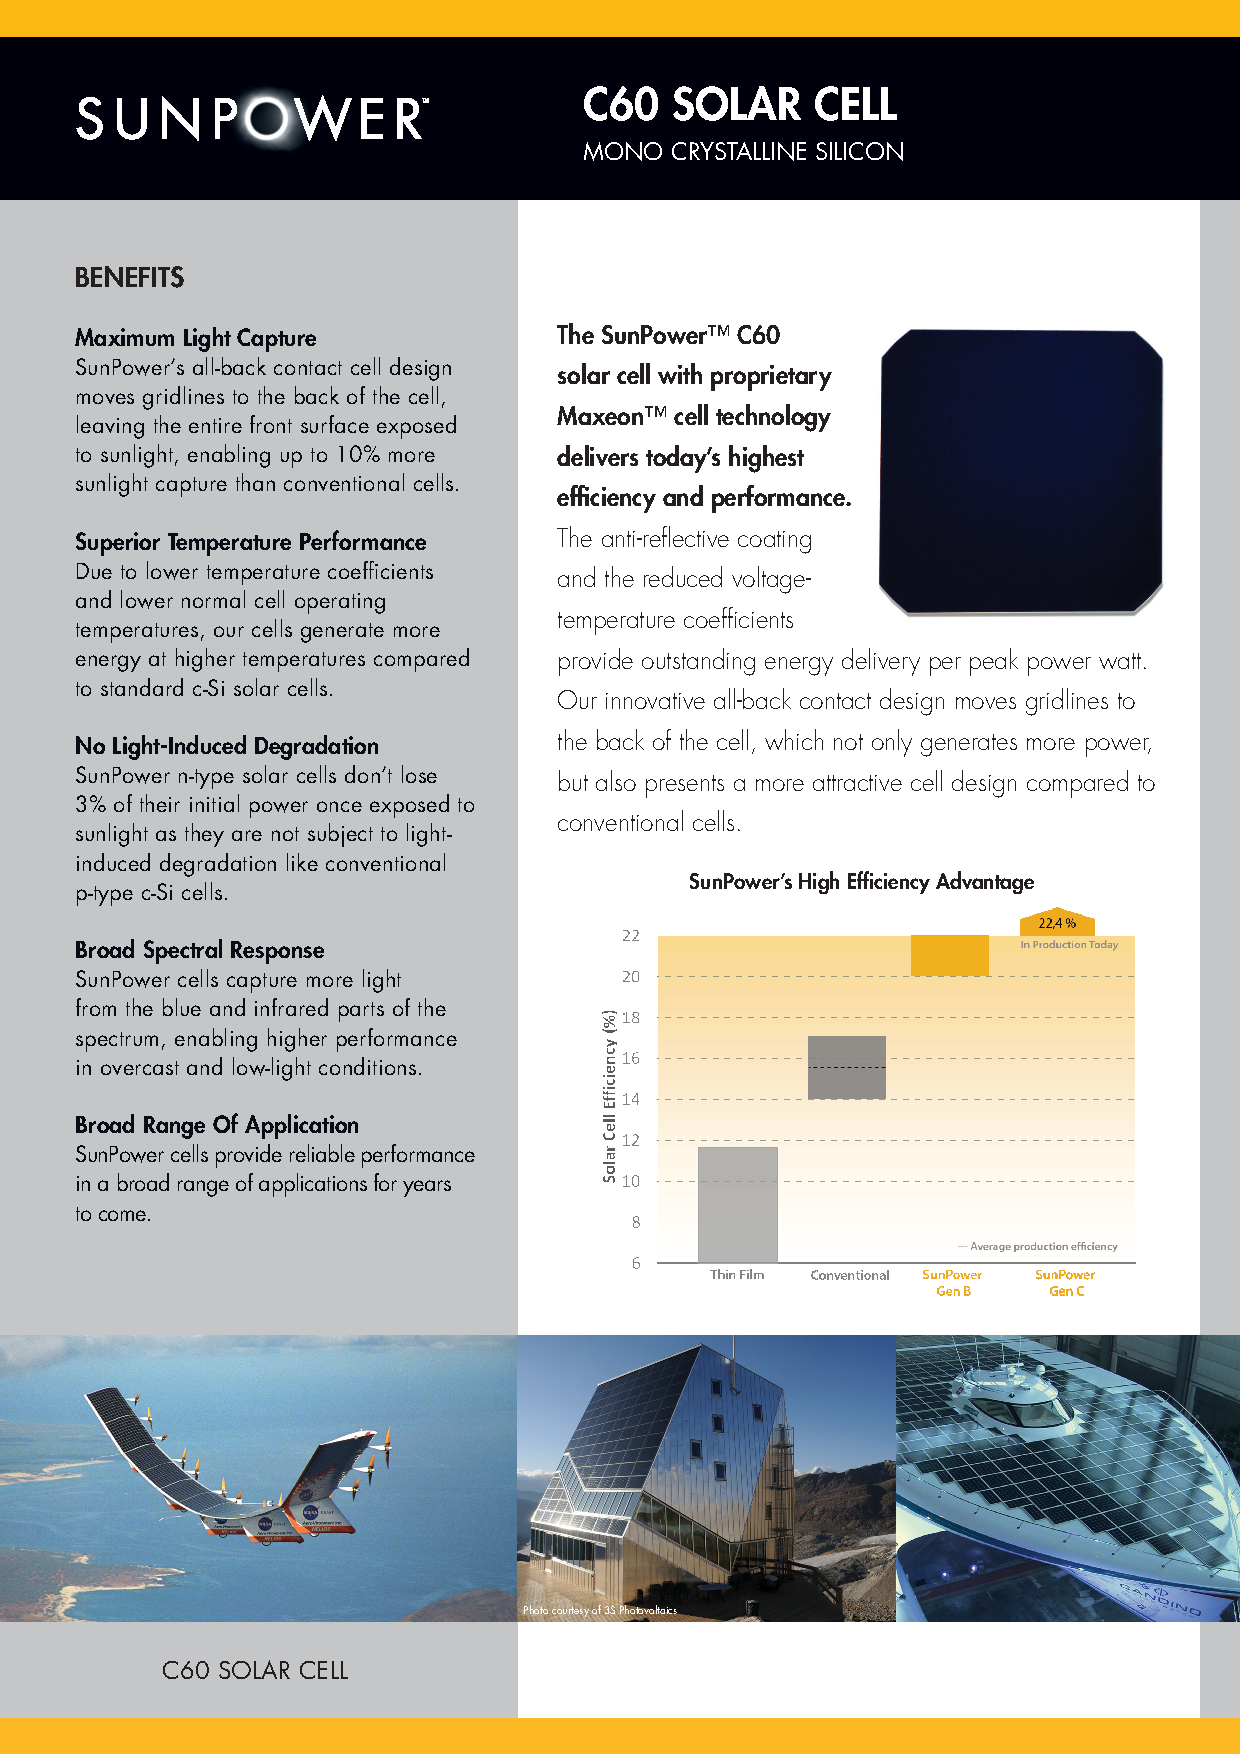
\includepdf[pages={1-2},nup=1x2,landscape=true]{Figures/SolarCell_Sunpower_C60.pdf}

 % file "Thesis_Appendix_B.tex"
%\cleardoublepage

% ----------------------------------------------------------------------
\end{document}
% ----------------------------------------------------------------------

